\documentclass{article}
\usepackage[utf8]{inputenc}
\usepackage{enumitem}
\usepackage{amsfonts}
\usepackage{amssymb}
\usepackage{hyperref}
\usepackage{wrapfig}
\usepackage{graphicx}
\graphicspath{ {images/} }

\hypersetup{
    colorlinks=true,
    linkcolor=black,
    filecolor=black,
    urlcolor=black,
    citecolor=black,
}

\title{
MIDA
\\
User Testing Guide
\\
\textit{Multi-Modality} vs \textit{AI-Assisted}
\\
Assistant Introduction
}

\author{
Francisco Maria Calisto\\
\texttt{francisco.calisto@tecnico.ulisboa.pt}
}

\date{07/03/2019}

\begin{document}

\maketitle

\textbf{Prototype:} \hyperlink{https://github.com/MIMBCD-UI/prototype-multi-modality}{prototype-multi-modality} \hfill \textbf{Version:} \hyperlink{https://github.com/MIMBCD-UI/prototype-multi-modality/releases/tag/v1.0.1-alpha}{v1.0.1-alpha}

\textbf{Milestone:} \hyperlink{https://github.com/MIMBCD-UI/prototype-breast-screening/milestone/1}{1.2.0-beta} \hfill \textbf{Release:} \hyperlink{https://github.com/MIMBCD-UI/prototype-breast-screening/releases/tag/v1.2.0-beta}{v1.2.0-beta}

\hfill

\textbf{Prototype:} \hyperlink{https://github.com/mida-project/prototype-multi-modality-assistant}{prototype-multi-modality-assistant} \hfill \textbf{Version:} \hyperlink{https://github.com/mida-project/prototype-multi-modality-assistant/releases/tag/v1.2.0-alpha}{v1.2.0-alpha}

\textbf{Milestone:} \hyperlink{https://github.com/mida-project/prototype-multi-modality-assistant/milestone/2}{1.2.0-alpha} \hfill \textbf{Release:} \hyperlink{https://github.com/mida-project/prototype-multi-modality-assistant/releases/tag/v1.2.0-alpha}{v1.2.0-alpha}

\hfill

\textbf{DICOM:} \hyperlink{https://github.com/MIMBCD-UI/dicom-server}{dicom-server}

\textbf{Commit:} \hyperlink{https://github.com/MIMBCD-UI/dicom-server/tree/80191e9941c24043c7f612b2dadcd415c060bf96}{80191e9941c24043c7f612b2dadcd415c060bf96}

\hfill

\textbf{Depl. Env.:} Localhost \hfill \textbf{Depl. Server:} Localhost

\textbf{Link:} \hyperlink{http://www.breastscreening.io/dashboard/}{breastscreening.io/dashboard}

\hfill

\textbf{Main Server:} \hyperlink{http://localhost:8486/src/public/index.html}{Localhost} \hfill \textbf{Port:} 8486

\textbf{Private IP:} \hyperlink{http://localhost:8486/src/public/index.html}{localhost} \hfill \textbf{Public IP:} \hyperlink{http://localhost:8486/src/public/index.html}{localhost}

\textbf{Private Domain:} \hyperlink{http://localhost:8486/src/public/index.html}{localhost}

\hfill

\textbf{DICOM Server:} \hyperlink{http://localhost:8448/app/explorer.html}{Localhost} \hfill \textbf{Port:} 8448

\textbf{Private IP:} \hyperlink{http://localhost:8448/app/explorer.html}{localhost} \hfill \textbf{Public IP:} \hyperlink{http://localhost:8448/app/explorer.html}{localhost}

\textbf{Private Domain:} \hyperlink{http://localhost:8448/app/explorer.html}{localhost} \hfill \textbf{From:} 8448

\clearpage

%%%%%%%%%%%%%%%%%%%%%%%%%%%%%%%%%%%%%%%%%%%%%%%%%%%
%                                                 %
%                     SECTION                     %
%                                                 %
%%%%%%%%%%%%%%%%%%%%%%%%%%%%%%%%%%%%%%%%%%%%%%%%%%%

\section{Introduction}
\label{sec:sec001}

This document aims to describe the protocol and guidelines of the presented information. We perform a set of tests in the scope of \hyperlink{https://github.com/MIMBCD-UI/prototype-multi-modality/releases/tag/v1.0.1-alpha}{v1.0.1-alpha}, \hyperlink{https://github.com/mida-project/prototype-multi-modality-assistant/releases/tag/v1.2.0-alpha}{v1.2.0-alpha} and \hyperlink{https://github.com/mida-project/prototype-heatmap/releases/tag/v1.2.0-alpha}{v1.2.0-alpha} versions from {\it \hyperlink{https://github.com/MIMBCD-UI/prototype-multi-modality}{Multi-Modality}}, {\it \hyperlink{https://github.com/mida-project/prototype-multi-modality-assistant}{Assistant}} and {\it \hyperlink{https://github.com/mida-project/prototype-heatmap}{Heatmap}} prototypes, respectively. The repositories are part of the \hyperlink{https://mida-project.github.io/}{MIDA} project using traditional devices (mouse and keyboard). The goal of the test is to compare each prototype, measuring the user performance, efficiency and efficacy metrics. The sessions will be recorded via video on a computer and using an interaction record, while triggering event tools. It is guaranteed the confidentiality of the recordings, which will be used only for academic purpose. Also, we will use an \hyperlink{https://gaming.tobii.com/products/}{eye-tracking device} to track the participant's eye movements during the breast cancer diagnosis.

Dividing the activity session into three distinct phases (\textbf{Pha\textit{N}.}, where \textit{N}. is the \textit{n}th number of a limited series, $n \in \mathbb{N}$ $\forall$ $N = \{1, 2, 3\}$) per each three activities representing two different scenarios: \textit{Multi-Modality} (\textbf{Sce1.}) vs \textit{Assistant} (\textbf{Sce2.}). The first two phases took place on an \hyperlink{https://github.com/MIMBCD-UI/testing-guide-breast/tree/master/samples/test_4}{early stage} of the \textit{User Tests}, while we were focus to publish the results on a near future. The third phase, will cover the hereby \textit{User Testing Guide}. Still, we will describe, as follows, the overall of the three phases to give higher contextualization.

Each scenario (\textbf{Sce\textit{M}.}, where \textit{M}. is the \textit{m}th number of a limited series, $m \in \mathbb{N}$ $\forall$ $M = \{1, 2\}$) will have three random patients (\textit{i.e.}, \textbf{Pat1.}, \textbf{Pat2.} or \textbf{Pat3.}) from a set of 50 total number of patients. For each patient (\textbf{Pat\textit{P}.}, where \textit{P}. is the \textit{p}th number of a limited series, $p \in \mathbb{N}$ $\forall$ $P = \{1, 2, 3\}$), we will choose it from the total set of patients randomly. We do it as follows, let \textit{R} be a random variable (\textbf{Rdm}) following the discrete uniform distribution as $r_{1}, r_{2}, r_{3} \in \mathbb{N}$ $\forall$ $R = \{1, ..., 50\}$. While $Pat1. = Rdm_{r_{1}}$ $\wedge$ $Pat2. = Rdm_{r_{2}}$ $\wedge$ $Pat3. = Rdm_{r_{3}}$ as far as $r_{1}$ $\neq$ $r_{2}$ $\neq$ $r_{3}$ is \textit{True}. In both two scenarios, \textit{i.e.}, \textit{Multi-Modality} (\textbf{Sce1.}) and \textit{Assistant} (\textbf{Sce2.}), by supporting our traditional devices, the interaction is made with mouse and keyboard. Participants will classify each patient by using the \hyperlink{https://en.wikipedia.org/wiki/BI-RADS}{BIRADS}~\cite{balleyguier2007birads}. We will do several small questionnaires at the end of each scenario using \hyperlink{https://en.wikipedia.org/wiki/NASA-TLX}{NASA-TLX}~\cite{ramkumar2017using}, \hyperlink{https://en.wikipedia.org/wiki/System_usability_scale}{System Usability Scale (SUS)}~\cite{orfanou2015perceived} and measuring the breast severity, as well as patients' pathologies.

Describing each phase, the first phase is nominated as \textbf{Pha1. User Characterization}. It is the \hyperlink{https://docs.google.com/spreadsheets/d/1h-4neEo3RbYsJs3JHBGvogHCvz3UFnMvsmoernfCuDU/edit?usp=sharing}{Demographic Questionnaire}, supporting our several characterizations of the participant profile. For the major number of participants, this phase was committed on an \hyperlink{https://github.com/MIMBCD-UI/testing-guide-breast/tree/master/samples/test_4}{early stage}, as stated above. The \textbf{Pha1.} phase has three activities (\textbf{Act\textit{A}.}, where \textit{A}. is the \textit{a}th number of a limited series, $a \in \mathbb{N}$) which are described as follows. The first activity, named as \textbf{Act1. Consent Form}, serves the purpose of providing participants information about privacy of the data and accept to proceed the test. The second activity, named as \textbf{Act2. Study Introduction}, serves the purpose of giving participants project contextualization and task awareness. Last but not least, the third activity of \textbf{Pha1.} phase, called as \textbf{Act3. Demographic Questionnaires}, is where participants fill a set of surveys regarding their characterization as a participant.

The second phase, nominated as \textbf{Pha2. Improving Visualization}, is also related with our later \href{https://github.com/MIMBCD-UI/prototype-breast-screening/wiki/User-Research#user-test-evaluations-}{User Test Evaluations}, corresponding to the tests done for the \textit{Multi-Modality} (\textbf{Sce1.}) scenario. At this \textbf{Pha2.} we divided it into two activities: (1) \textbf{Act4. Scenario Introduction} activity; and (2) \textbf{Act5. Scenario Evaluation} activity. Both applied for the {\bf Sce1.} scenario.

The first \textbf{Act4.} activity, aims at providing participants information about what tasks they will do. Each task represents the diagnostic of each patient, while we named it as \textbf{Act5. Scenario Evaluation} activity of the {\bf Sce1.} scenario. An intermediate \textbf{Act6. Scenario Exploration} was created, aiming at providing participants a free opportunity to explore the system and give opinion in regard for {\bf Pha2.} phase. It will be important information for the {\it Qualitative Analysis (QA)}. Finally, the \textbf{Act7. Post-task Scenario Questions}, of the {\bf Sce1.} scenario, will be a set of \textit{post-task} questions for {\bf Pha2.} phase.

Finally, and most importantly, the third phase, nominated as \textbf{Pha3. Assistant Establishment} phase, is where participants proceed for the diagnosis of the respective three, \textit{i.e.}, \textbf{Pat1.}, \textbf{Pat2.} and \textbf{Pat3.} patients. It is here, where we will also verify if our proposed designs impact \cite{amershi2019guidelines, kocielnik2019will} on user expectations, as intended, specifically as outlined by our several \textit{Hypotheses} for the respective \textit{Research Questions} (Section \ref{sec:sec006}). We did it in regard to the novel introduction of an \textit{AI-Assisted} system, calling it as \textit{BreastScreening}~\cite{calistobreastscreening}.

On the {\bf Pha3.} phase, we will measure the participants expectations concerning the \textit{AI-Assisted} system applying an \textbf{Act8. Scenario Expectations} activity for the {\bf Sce2.} scenario. The next \textbf{Act4.  Scenario Introduction} activity of the {\bf Sce2.} scenario, will be the introductory information about \textit{AI-Assisted} system and what feature are covered by the system. The \textbf{Act5. Scenario Evaluation} activity of the {\bf Sce2.} scenario, represents the diagnostic of each patient, but this time with support of our novel \textit{AI-Assisted} recommendations and explainability. Another intermediate \textbf{Act6. Scenario Exploration} of the {\bf Sce2.} scenario, in regard for the {\bf Pha3.} phase, where also, it will generate important information for our {\it QA}. Finally, the \textbf{Act7. Post-task Scenario Questions} of the {\bf Sce2.} scenario, will be a set of \textit{post-task} questions.

For this {\it User Testing Guide}, we used three prototype repositories, \textit{i.e.}, \textit{\hyperlink{https://github.com/MIMBCD-UI/prototype-multi-modality}{Multi-Modality}}, \textit{\hyperlink{https://github.com/mida-project/prototype-multi-modality-assistant}{Assistant}} and \textit{\hyperlink{https://github.com/mida-project/prototype-heatmap}{Heatmap}} prototypes. The prototypes are similar mirrors of the \hyperlink{https://github.com/MIMBCD-UI/prototype-breast-screening}{prototype-breast-screening} with major changes. It is further described.

The first, \textit{i.e.}, {\it \hyperlink{https://github.com/MIMBCD-UI/prototype-multi-modality}{Multi-Modality}} prototype, aims at providing clinicians a \textit{Multi-Modality} strategy view. The \textit{Multi-Modality} view, gives clinicians the possibility for visualizing three modalities: (i) \hyperlink{https://medical-dictionary.thefreedictionary.com/mammography}{MammoGraphy (MG)}, both \hyperlink{https://medical-dictionary.thefreedictionary.com/craniocaudal}{CranioCaudal (CC)} and \hyperlink{https://www.thefreedictionary.com/mediolateral}{MedioLateral Oblique (MLO)} views; \hyperlink{https://www.thefreedictionary.com/UltraSound}{UltraSound (US)}; and \hyperlink{https://www.thefreedictionary.com/Magnetic+Resonance+Imaging}{Magnetic Resonance Imaging (MRI)}. It corresponds to the \textbf{Sce1.} scenario of both \textbf{Act4.}, \textbf{Act5.} and \textbf{Act6.} activities at \textbf{Pha2.} phase.

Second and third repositories, \textit{i.e.}, from both \hyperlink{https://github.com/mida-project/prototype-multi-modality-assistant}{prototype-multi-modality-assistant} and \hyperlink{https://github.com/mida-project/prototype-heatmap}{prototype-heatmap} repositories, aims at providing clinicians a recommendation system regarding our \textit{AI-Assistive} techniques. Those techniques, will provide clinicians a twofold: (a) the opportunity of receive automatic recommendations concerning breast severities (\hyperlink{https://en.wikipedia.org/wiki/BI-RADS}{BIRADS}) of the patients; and (b) giving clinicians explainability (\hyperlink{https://www.darpa.mil/program/explainable-artificial-intelligence}{XAI})~\cite{gunning2017explainable, holzinger2017we} of those results.

The automatic recommendations will be covered by the \hyperlink{https://github.com/mida-project/prototype-multi-modality-assistant}{prototype-multi-modality-assistant} repository, while the explainability will be covered by the \hyperlink{https://github.com/mida-project/prototype-heatmap}{prototype-heatmap} repository. Both techniques are corresponding to the \textbf{Sce2.} scenario of \textbf{Act4.}, \textbf{Act5.}, \textbf{Act6.}, \textbf{Act7.} and \textbf{Act8.} activities at the \textbf{Pha3.} phase.
%%%%%%%%%%%%%%%%%%%%%%%%%%%%%%%%%%%%%%%%%%%%%%%%%%%
%                                                 %
%                     SECTION                     %
%                                                 %
%%%%%%%%%%%%%%%%%%%%%%%%%%%%%%%%%%%%%%%%%%%%%%%%%%%

\section{Description}
\label{sec:sec002}

To verify our work, we identified measurable and explicit targets. By having several goals, including that a value percentage of the users should be able to operate the tasks without the need of help. On the same rate value, the user should be able to start and complete the medical diagnosis tasks over the system with little errors or mitigating those errors. Measuring the expected number of errors with a relation between our laboratory pilot tests. On the laboratory pilot tests we aim to test our prototypes with researchers. The Researchers are in the context of the system and know well the functionalities so that we need to expect a percentage value over their results compared to clinicians and not the same benefits. Last but not least, both users (researchers and clinicians) should be able to understand in a similar time amount the meaning of all visible controls. By the similar amount of time, it is expected to have a variance of the percentage value between researchers and clinicians of the same value percentage of the early goals described in this paragraph.

We tested each objective in early laboratory and field tests so that we could take the appropriate corrective actions. Also, we expect to run early field tests with researchers and clinicians to highlight issues that we overlooked and ignored during the prototyping phase. To support interaction use by the clinicians, we will try to emphasise several key factors on our user tests. The tasks must be simple, low intrusive, support for natural interaction and the system must always give visibility and the task current-state.

\clearpage

%%%%%%%%%%%%%%%%%%%%%%%%%%%%%%%%%%%%%%%%%%%%%%%%%%%
%                                                 %
%                     SECTION                     %
%                                                 %
%%%%%%%%%%%%%%%%%%%%%%%%%%%%%%%%%%%%%%%%%%%%%%%%%%%

\subsection{Devices}

Traditional interaction remains the most common way to interact with user interfaces in a clinical environment. Unfortunately, most of this interaction is made by low profile equipment that makes users produce more errors and take more time interacting with those user interfaces.

On Figure \ref{fig:patient_list} the user can select the list of patients. The list has a table with several patient information. The first column is the \textit{Patient ID}; we used it as an identifier of the patient. That way we can have anonymised information with no reference to the patient name. The second column is the \textit{Study Date}, the third column is the \textit{Modality} of the used \textbf{DICOM} image, the fourth column is the \textit{Study Description} of the used study and the last column is the number of \textit{Images}.

%%%%%%%%%%%%%%%%%%%%%%%%%%%%%%%%%%%%%%%%%%%%%%%%%%%

\hfill

\begin{figure}[h]
\centering
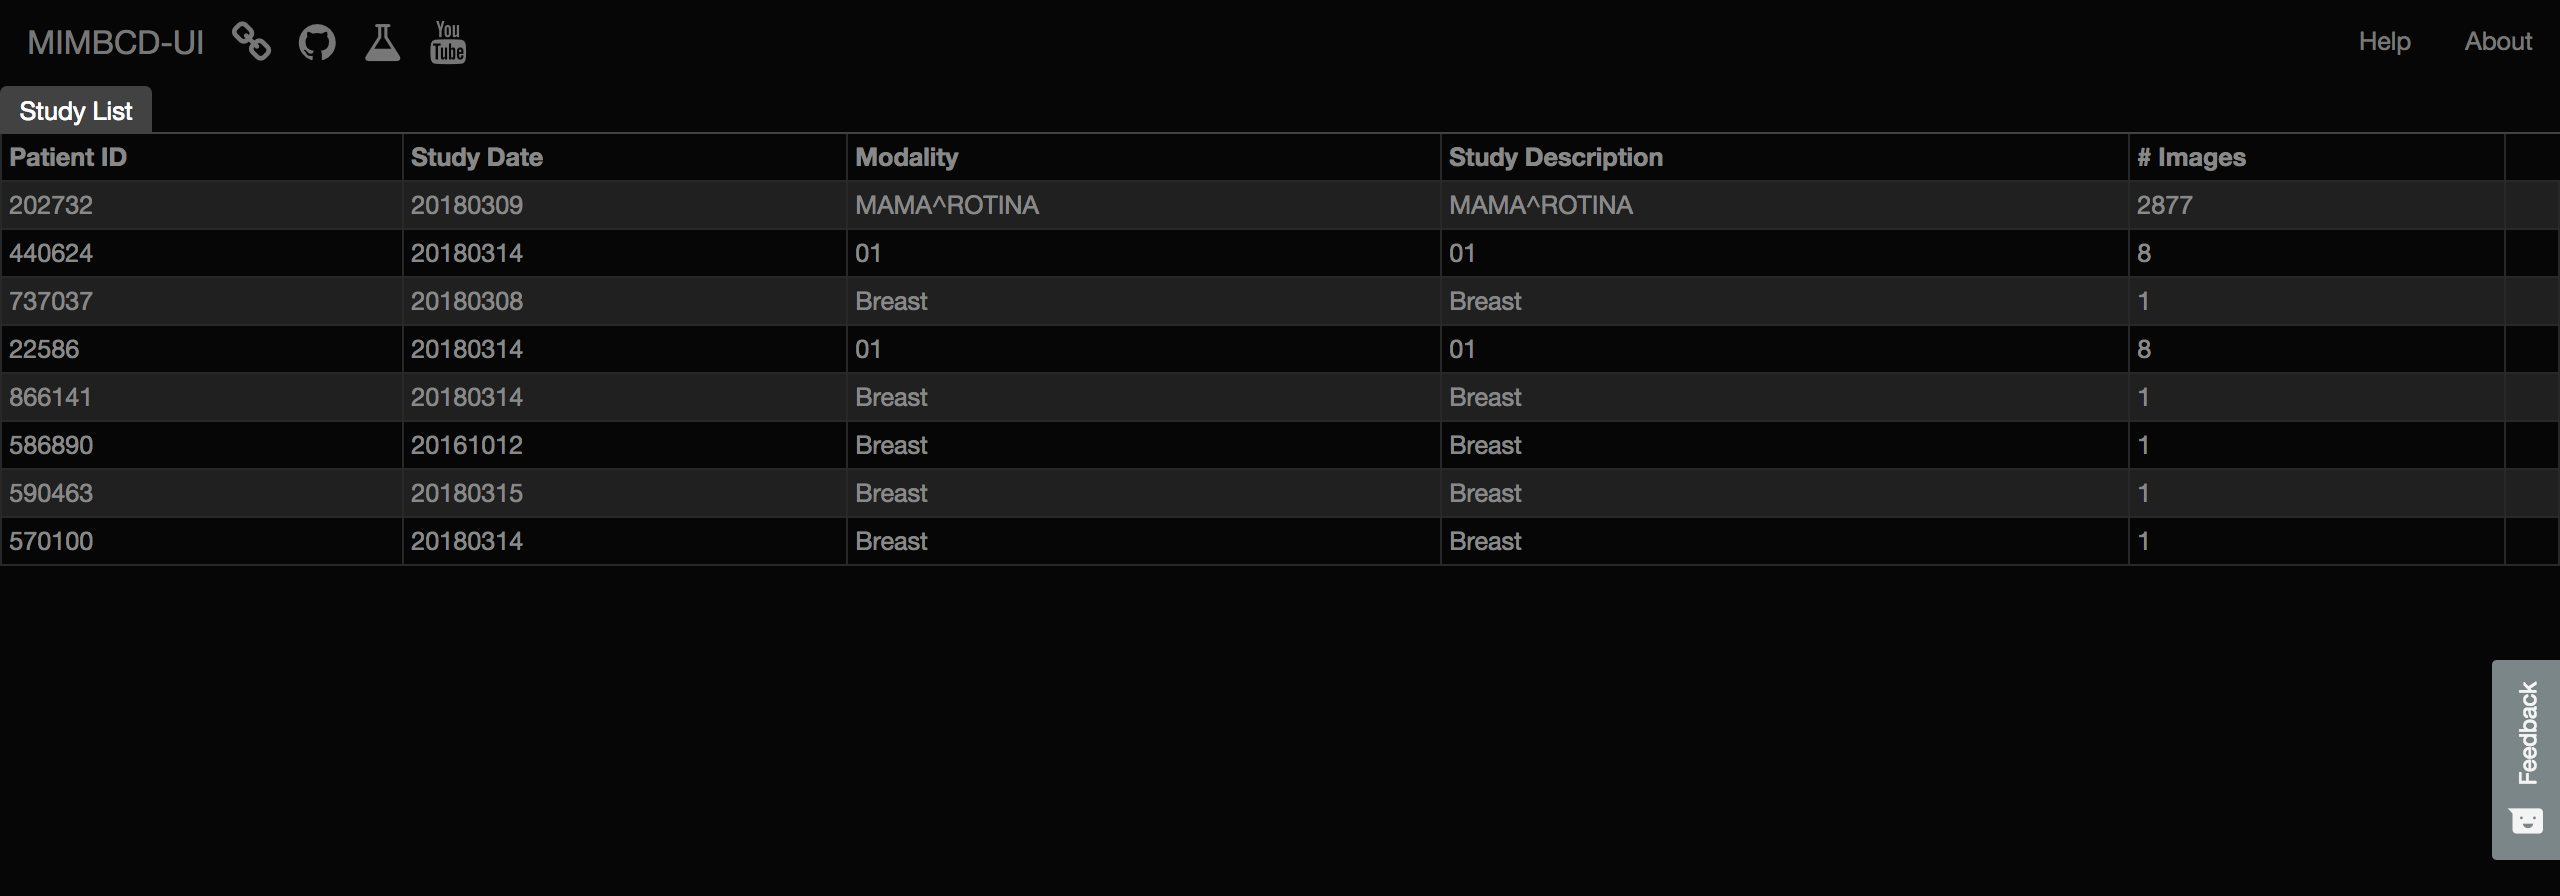
\includegraphics[width=\textwidth]{patient_list}
\caption{List of Patients.}
\label{fig:patient_list}
\end{figure}

\hfill

%%%%%%%%%%%%%%%%%%%%%%%%%%%%%%%%%%%%%%%%%%%%%%%%%%%

As we can see in Figure \ref{fig:image_viewer}, it shows the first task in our User Interface (UI), where the patient's breasts are on a small left column. The options are in a short row near of the viewport and described below. We also have the tabs where the user can change the patient. The centre viewport shows the \textbf{DICOM} image, and it can be configured to display a number up to four \textbf{DICOM} images at the same time. The viewport has some text information on it (yellow) with the details of the metadata. Nevertheless, the \textbf{Assistant} suggestions are shown on the top-right corner of the system.

\clearpage

%%%%%%%%%%%%%%%%%%%%%%%%%%%%%%%%%%%%%%%%%%%%%%%%%%%

\hfill

\begin{figure}[h]
\centering
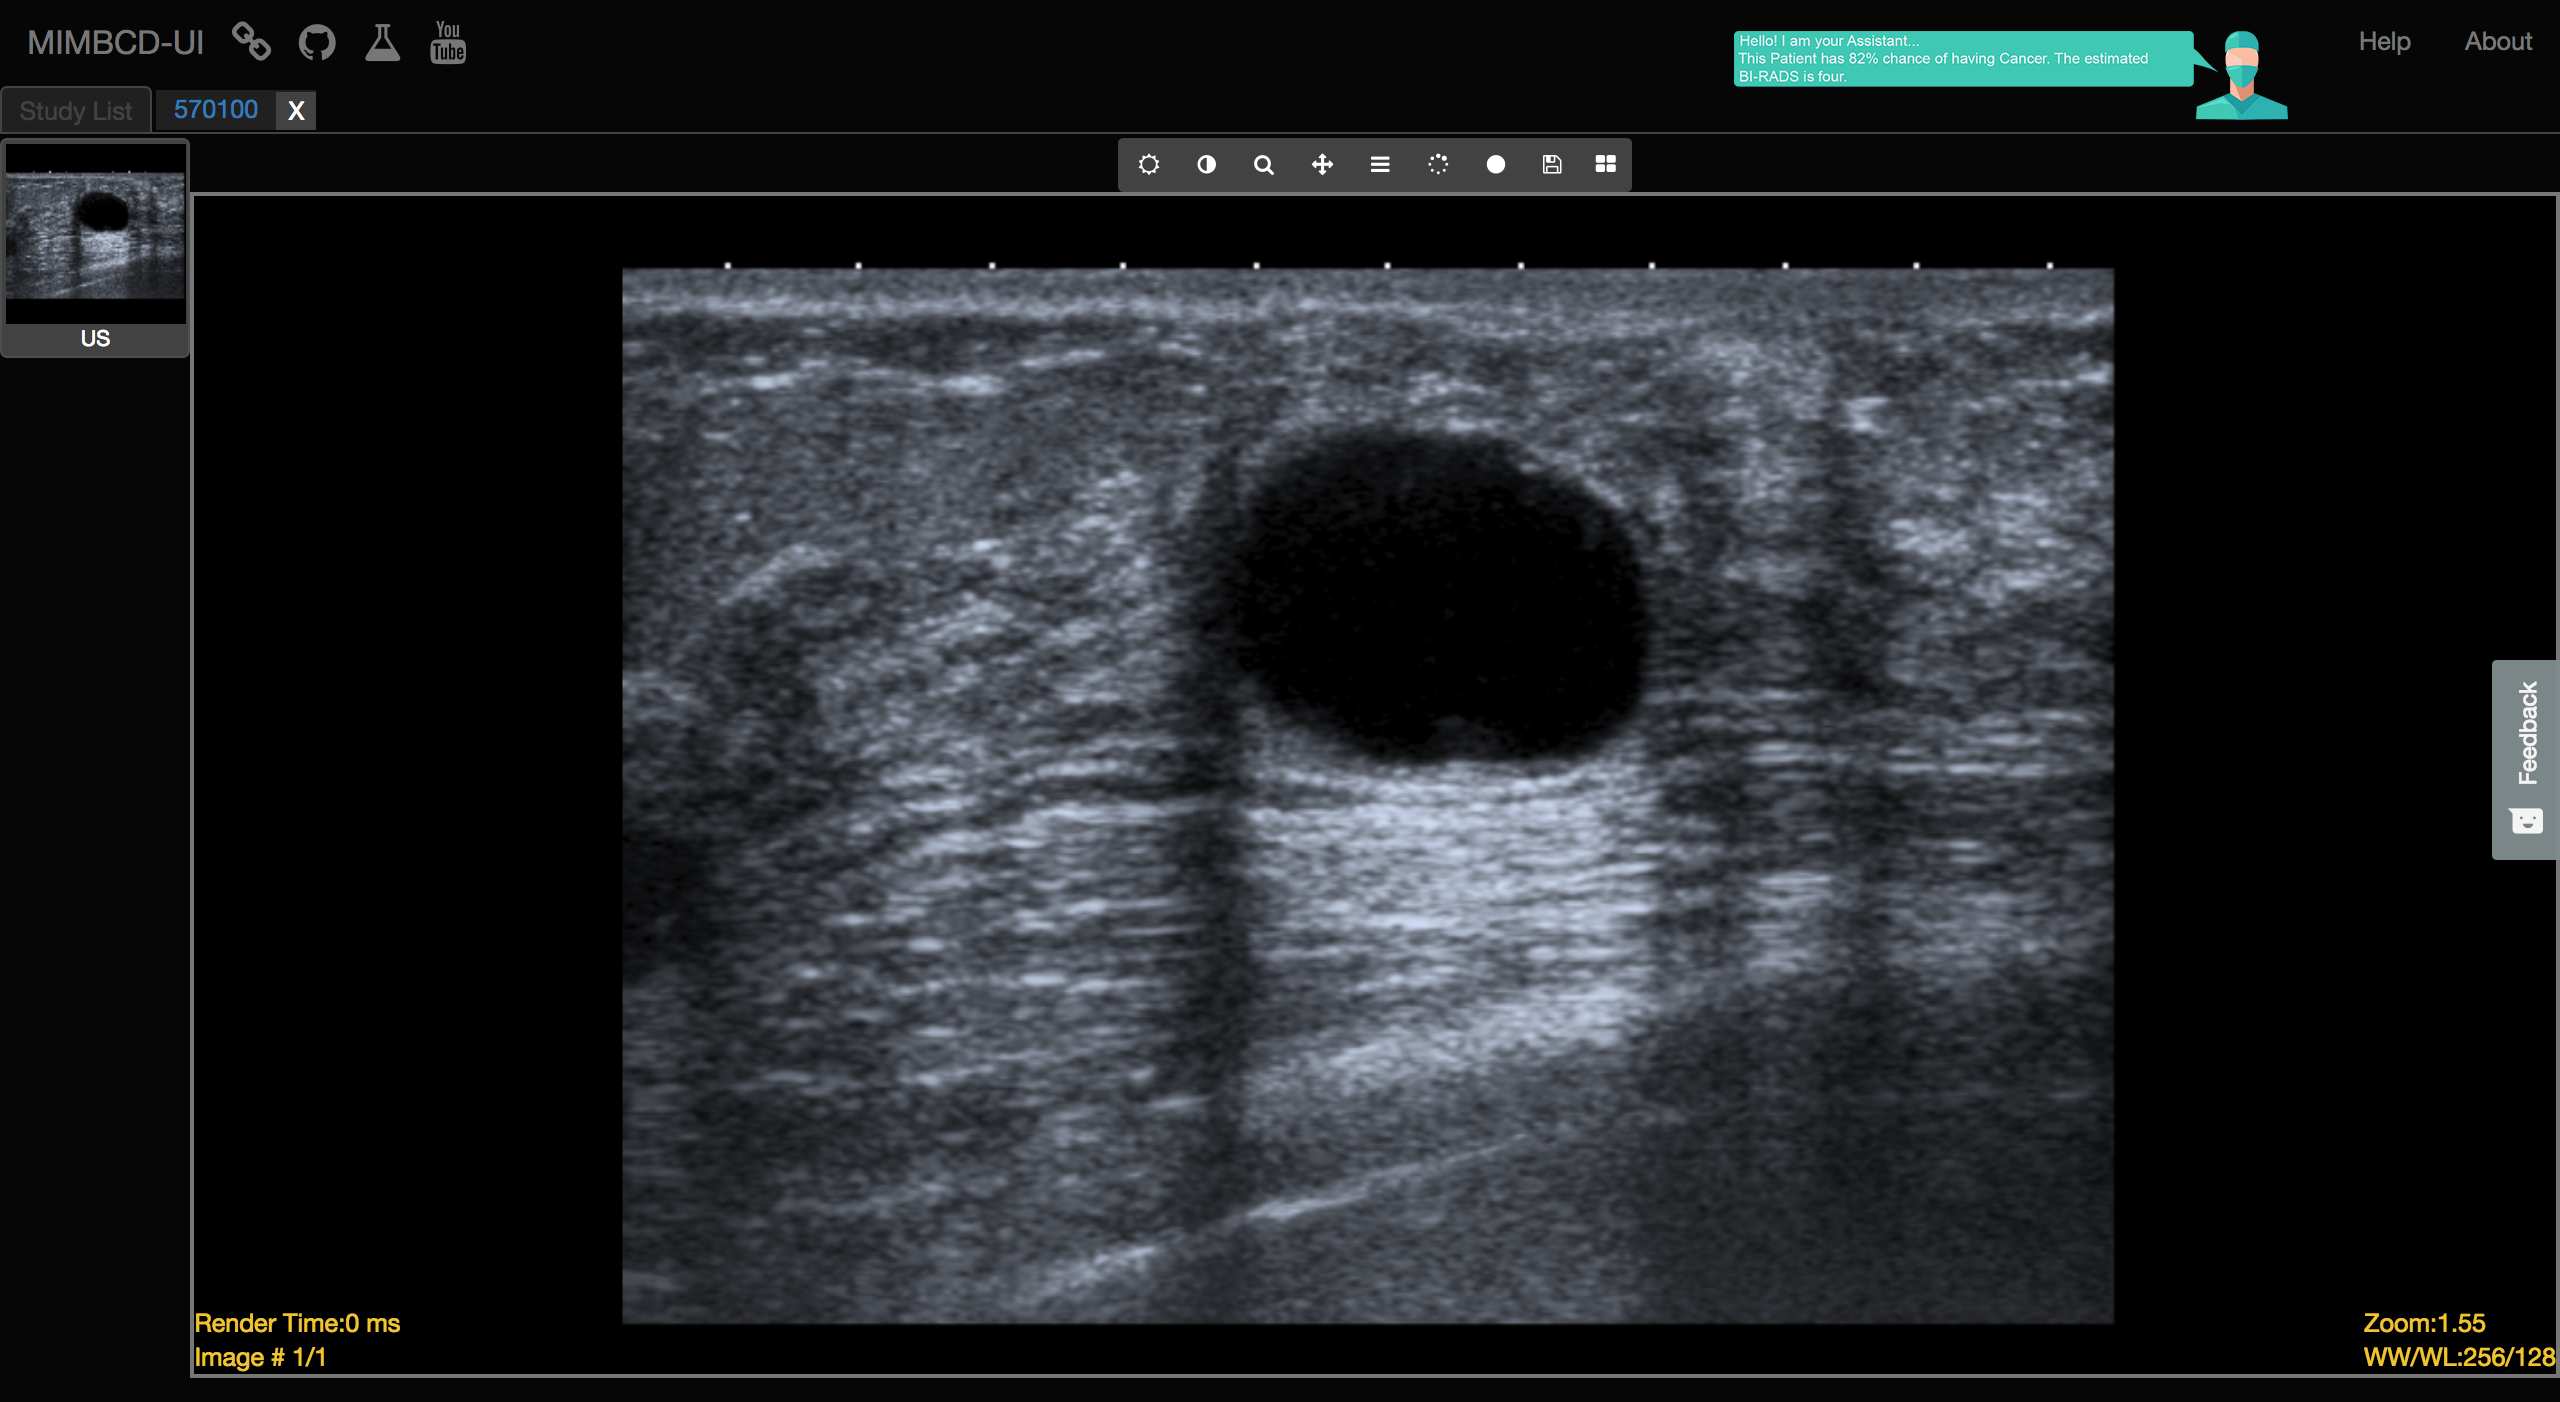
\includegraphics[width=\textwidth]{image_viewer}
\caption{Viewer of the \textbf{DICOM} images.}
\label{fig:image_viewer}
\end{figure}

\hfill

%%%%%%%%%%%%%%%%%%%%%%%%%%%%%%%%%%%%%%%%%%%%%%%%%%%

Manual annotation~\citation{cao2015collaborative} is adopted by us thanks to Freehand ROI and Probe annotation features, both from \hyperlink{https://cornerstonejs.org/}{CornerstoneJS}. According to the \hyperlink{https://cornerstonejs.org/}{CornerstoneJS} Library, the user can create an annotation by setting up consecutive landmarks around a Region of Interest (ROI). The markers finish a lesion annotation when it interconnects the historical. Additional features available in our User Interface (UI) includes on-demand increment of the number of landmarks, and throw transformations of the shape of an annotation.

\clearpage

%%%%%%%%%%%%%%%%%%%%%%%%%%%%%%%%%%%%%%%%%%%%%%%%%%%
%                                                 %
%                     SECTION                     %
%                                                 %
%%%%%%%%%%%%%%%%%%%%%%%%%%%%%%%%%%%%%%%%%%%%%%%%%%%

\subsection{User Interactions}

The systems have several buttons (Figure \ref{fig:toolbar}) that allows the user to interact or access to a set of user interface features. Each item of the following list represents each metaphoric icon of Figure \ref{fig:toolbar}.

%%%%%%%%%%%%%%%%%%%%%%%%%%%%%%%%%%%%%%%%%%%%%%%%%%%

\hfill

\begin{figure}[h]
\centering

\includegraphics[width=\textwidth]{toolbar}
\caption{Toolbar of the System available features.}
\label{fig:toolbar}
\end{figure}

\hfill

%%%%%%%%%%%%%%%%%%%%%%%%%%%%%%%%%%%%%%%%%%%%%%%%%%%

\hfill

The buttons are (from left to right of Figure \ref{fig:toolbar}) as follows:

\hfill

\begin{itemize}
\item WW/WC
\item Invert
\item Zoom
\item Pan
\item Stack Scroll
\item Freehand
\item Probe
\item Save
\item Window Controller
\end{itemize}

\hfill

\clearpage

%%%%%%%%%%%%%%%%%%%%%%%%%%%%%%%%%%%%%%%%%%%%%%%%%%%
%                                                 %
%                     SECTION                     %
%                                                 %
%%%%%%%%%%%%%%%%%%%%%%%%%%%%%%%%%%%%%%%%%%%%%%%%%%%

\subsection{Evaluation}

Introduction of AI \textbf{Assistant} agents are significant factors which can naturally affect the performance of a medical workflow. While some prior studies \cite{Calisto:2017:TTM:3132272.3134111, calistobreastscreening, calisto2017mimbcdui} have investigated the functionality of healthcare systems, the \textit{AI-Assisted} acceptability has mostly been overlooked in the existing Health Informatics (HI) literature regarding a Human-Computer Interaction (HCI).

The following Table \ref{table:usability_evaluation_questions} is presenting seven evaluation questions to have in mind during evaluation. The purpose of this questions is to facilitate systematic user studies regarding our novel \textbf{Assistant} in a clinical environment and support user stimulation for the introduction of \textit{AI-Assisted} methods. The proposed issues involve various aspects of workflow combined with either need for satisfaction or division of attention.

\hfill

\begin{table}[h]
\centering
\begin{tabular}{l|l}
Number & Issues of Content \& Key Questions                    	 \\ \hline
1      & How would the user describe the potential adoption of   \\
       & \textit{AI-Assisted} methods on the Health Institution? \\ \hline
2      & What are the user oppositions for \textit{AI-Assisted}	 \\
       & methods?                                                \\ \hline
3      & What examples of \textit{AI-Assisted} methods does the  \\
       & user know regarding the Health Institution?             \\ \hline
4      & What are the obstacles of the user's Health             \\
       & Institution?                                            \\ \hline
5      & What is more important for the \textit{AI-Assisted}     \\
       & information, the BIRADS or Pathology?                   \\ \hline
6      & Is it important for the user to have the feature of		 \\
       & Approve, Reject and Justify options?                    \\ \hline
7      & For the user's opinion, what are the aspects that       \\
       & influence the decision?                                 \\ \hline

\end{tabular}
\caption{Usability Evaluation Questions}
\label{table:usability_evaluation_questions}
\end{table}

\hfill

The influence of \textit{AI-Assisted}~\cite{goodfellow2016deep} is an important variable for our empirical analysis. In fact, the trust of the user increases when the user perceived that the \textbf{Assistant} is giving the right inputs and that there will be a consequent increase of the clinician trust in our system.

\clearpage

The first question, the \textit{How would the user describe the potential adoption of \textit{AI-Assisted} methods on the Health Institution?} question. For the second question, the \textit{What are the user oppositions for \textit{AI-Assisted} methods?} question, we aim to understand what are the user constrains regarding an AI adoption the the user's current workflow. Third, we intend to filter possible examples of the clinical applications of AI on the Health Institutions by asking \textit{What examples of \textit{AI-Assisted} methods does the user know regarding the Health Institution?} directly to the clinician. The fourth question, underlines the reasons why several obstacles are present on the Health Institution, with the question \textit{What are the obstacles of the user's Health Institution?} we can understand the challenges of achieving those issues and what are the solutions for surpass it. On the fifth question, where we ask \textit{What is more important for the \textit{AI-Assisted} information, the BIRADS or Pathology?}, we aim to understand what is more important for the user, the BIRADS or the Pathology~\cite{maicas2018pre} of the patient~\cite{elverici2015nonpalpable}. Almost last, the six question, where we ask for \textit{Is it important for the user to have the feature of \textbf{Approve}, \textbf{Reject} and \textbf{Justify} options?} is an important question to understand the feature needs and options. Last but not least, the seven question, \textit{For the user's opinion, what are the aspects that influence the decision?}, is where we will understand what is the most important information to show to the clinicians, therefore, we can more effectively and efficiently give more accurate information to the users.

To conclude this section, by doing this questions, we aim to support our user studies by giving our users, the clinicians, the opportunity of improving our empirical analysis regarding user's \textit{open answers}. However, the results should be treated with caution. Several bias exists since we are doing here an ambiguous approach.

\clearpage
%%%%%%%%%%%%%%%%%%%%%%%%%%%%%%%%%%%%%%%%%%%%%%%%%%%
%                                                 %
%                     SECTION                     %
%                                                 %
%%%%%%%%%%%%%%%%%%%%%%%%%%%%%%%%%%%%%%%%%%%%%%%%%%%

\section{Methodology}
\label{sec:sec003}

The hereby used prototypes are both \hyperlink{https://github.com/mida-project/prototype-multi-modality-assistant/releases/tag/v1.2.0-alpha}{v1.2.0-alpha} and \hyperlink{https://github.com/mida-project/prototype-heatmap/releases/tag/v1.2.0-alpha}{v1.2.0-alpha} versions of our \hyperlink{https://github.com/mida-project/prototype-multi-modality-assistant/}{prototype-multi-modality-assistant} and \hyperlink{https://github.com/mida-project/prototype-heatmap}{prototype-heatmap} repositories, respectively. The purpose of these prototypes is to involve an \textit{AI-Assisted} tool (\textit{Assistant}) for medical imaging at a breast screening diagnosis level. This \textit{Assistant} was created with a front-end and back-end architecture utilising common programming languages, libraries, frameworks and tools including \hyperlink{https://www.javascript.com/}{JavaScript (JS)}~\cite{flanagan2006javascript}, \hyperlink{https://nodejs.org/}{NodeJS}~\cite{wilson2018node}, \hyperlink{https://hammerjs.github.io/}{HammerJS}, \hyperlink{https://cornerstonejs.org/}{CornerstoneJS}~\cite{hostetter2018integration} and \hyperlink{https://www.orthanc-server.com/}{Orthanc}~\cite{Jodogne:ISBI2013}. For the Machine Learning (ML) and Deep Learning (DL)~\cite{ribeiro2017real, ribeiro2016real} component we will use several \hyperlink{https://www.mathworks.com/products/matlab.html}{MATLAB} technologies~\cite{vedaldi2015matconvnet}, promoting and feeding our Convolutional Neural Networks (CNN)~\cite{carneiro2015unregistered} and Deep Reenforcement Learning (DRL)~\cite{maicas2017deep} techniques. Other central component of this prototype is a web-based \hyperlink{https://www.sciencedirect.com/topics/medicine-and-dentistry/picture-archiving-and-communication-system}{PACS}~\cite{cooke2003picture} pairwise with ubicous web technologies and based on the \textbf{Open Source (OS)} \hyperlink{https://cornerstonejs.org/}{CornerstoneJS} library~\cite{feller2002understanding, hostetter2018integration}.

%%%%%%%%%%%%%%%%%%%%%%%%%%%%%%%%%%%%%%%%%%%%%%%%%%%
%                                                 %
%                     SECTION                     %
%                                                 %
%%%%%%%%%%%%%%%%%%%%%%%%%%%%%%%%%%%%%%%%%%%%%%%%%%%

\subsection{Environments}

This section describes the user environment over interaction, the so called \textbf{Radiology Room (RR)} (Figure \ref{fig:radioroom}). This guide is based on soft-copy diagnosis using computer workstations in their current reading room environment. It will be here where we take impressions regarding the efficacy of radiologists, and their recommendations based on their experience for improvements on the soft-copy reading environment. Several studies demonstrated~\cite{waite2017tired} that radiologist fatigue levels and performance are related to environmental factors such as number of false-negative and false-positives, in addition to workstation enhancements. Supported by this guide, our research aims to conduct an investigation for the several environmental variables and improvements regarding the potentially enhancement that an \textit{AI-Assisted} diagnosis could take in the \textbf{RR}. We expect to analyze the needed information and best solution to improve the workstation results.

%%%%%%%%%%%%%%%%%%%%%%%%%%%%%%%%%%%%%%%%%%%%%%%%%%%

\hfill

\begin{figure}[h]
\centering
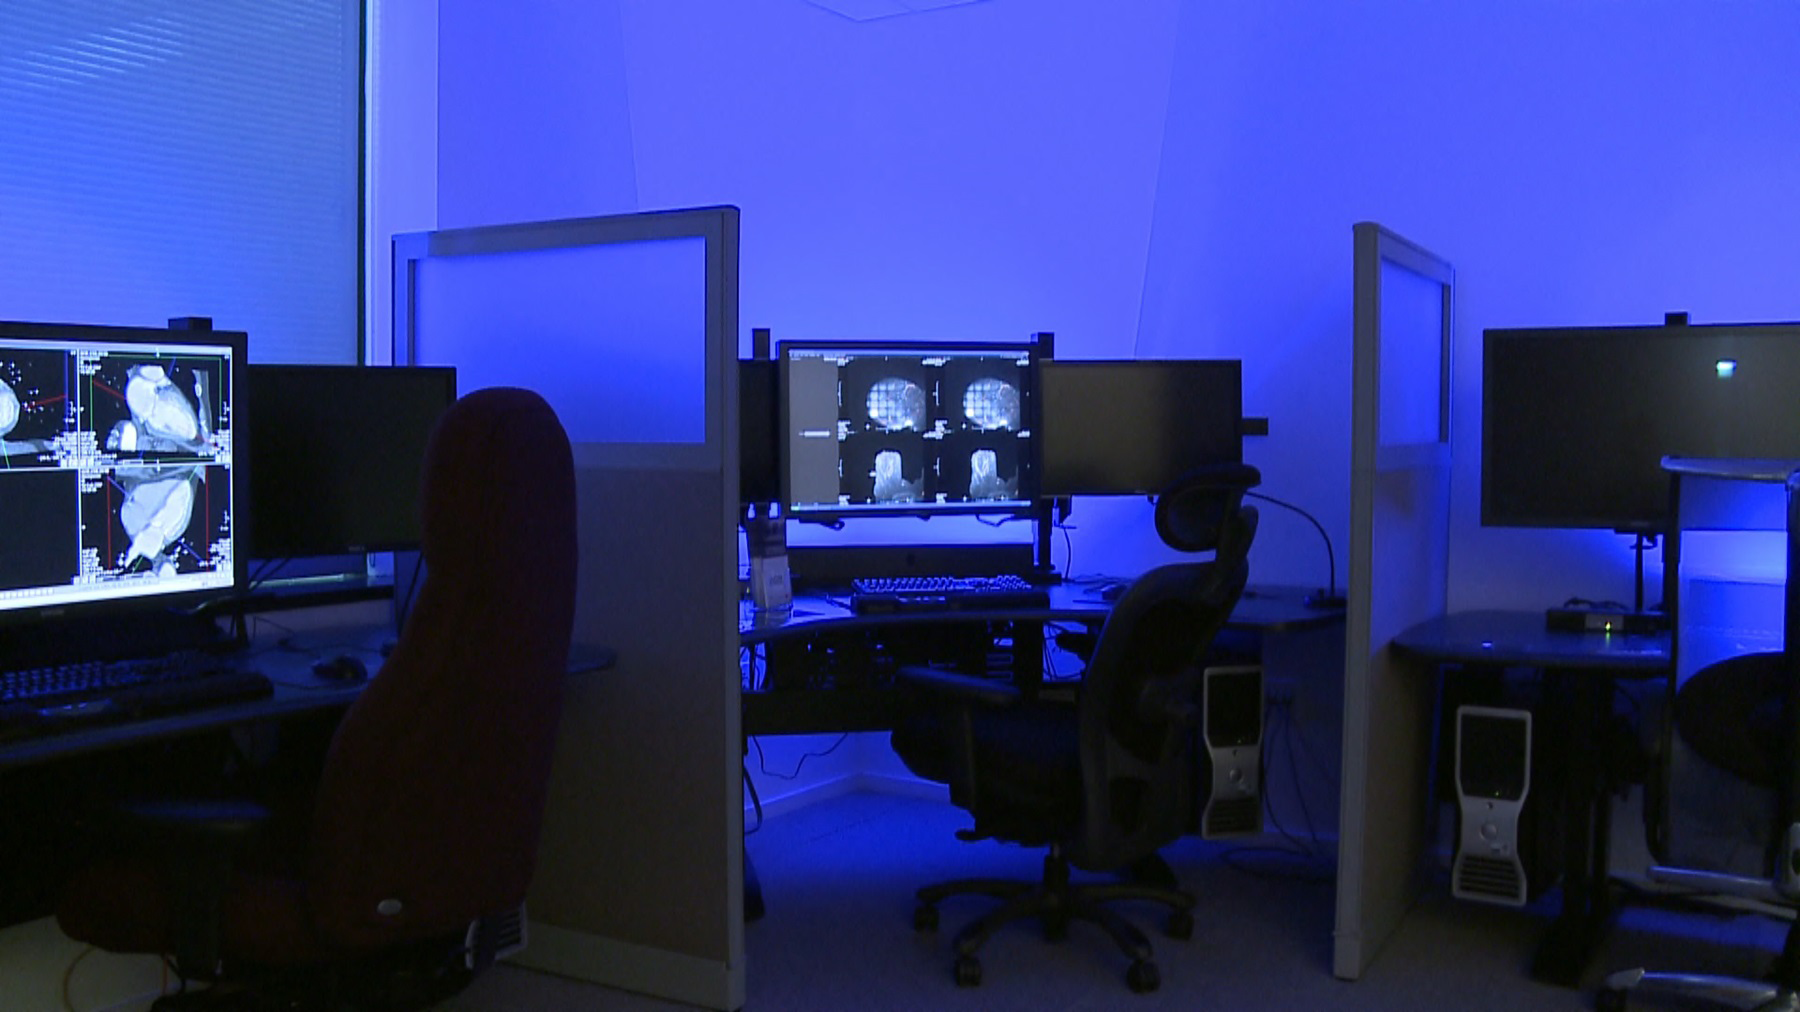
\includegraphics[width=\textwidth]{acr}
\caption{Radiology Room}
\label{fig:radioroom}
\end{figure}

\hfill

%%%%%%%%%%%%%%%%%%%%%%%%%%%%%%%%%%%%%%%%%%%%%%%%%%%

%%%%%%%%%%%%%%%%%%%%%%%%%%%%%%%%%%%%%%%%%%%%%%%%%%%
%                                                 %
%                     SECTION                     %
%                                                 %
%%%%%%%%%%%%%%%%%%%%%%%%%%%%%%%%%%%%%%%%%%%%%%%%%%%

\subsection{Participants}

The participants' responsibilities will be to attempt to complete a set of representative task scenarios presented to them in as efficient and timely a manner as possible, and to provide feedback regarding the usability and acceptability of an \textit{AI-Assisted} diagnosis. The participants will be directed to provide honest opinions regarding the user tests of the interacted systems, and to participate in post-session subjective questionnaires and debriefing.

%%%%%%%%%%%%%%%%%%%%%%%%%%%%%%%%%%%%%%%%%%%%%%%%%%%

%%%%%%%%%%%%%%%%%%%%%%%%%%%%%%%%%%%%%%%%%%%%%%%%%%%
%                                                 %
%                     SECTION                     %
%                                                 %
%%%%%%%%%%%%%%%%%%%%%%%%%%%%%%%%%%%%%%%%%%%%%%%%%%%

\subsection{Procedure}

Participants will take part in the tests at our formed institution protocols (\textit{e.g.}, \hyperlink{http://hff.min-saude.pt/}{Hospital Fernando Fonseca (HFF)}) with both \hyperlink{https://github.com/mida-project/prototype-multi-modality-assistant/releases/tag/v1.2.0-alpha}{v1.2.0-alpha} and \hyperlink{https://github.com/mida-project/prototype-heatmap/releases/tag/v1.2.0-alpha}{v1.2.0-alpha} versions of our \hyperlink{https://github.com/mida-project/prototype-multi-modality-assistant/}{prototype-multi-modality-assistant} and \hyperlink{https://github.com/mida-project/prototype-heatmap}{prototype-heatmap} repositories, respectively. The interaction with the system will be used in a typical \textbf{RR} environment. Note takers and data logger(s) will monitor the sessions for observation in the \textbf{RR}, connected by screen recording feed. The test sessions will be recorded and further analyzed.

The facilitator will brief the participants on the system features and instruct the participant that they are evaluating the system, rather than the facilitator evaluating the participant. Participants will sign an informed consent (\textbf{Pha1.} - \textbf{Act1.}) that acknowledges: the participation is voluntary, that participation can cease at any time, and that the session will be videotaped and eye tracked but their privacy of identification will be safeguarded. The facilitator will ask the participant if they have any questions.

\hfill

Participants will complete a pre-test demographic (\textbf{Pha1.} - \textbf{Act3.}) and background information (\textbf{Pha1.} - \textbf{Act2.}) questionnaires. The facilitator will explain that the amount of time taken to complete the test task, will be measured and that exploratory behavior outside the task flow should not occur until after task completion. At the start of each task, the participant will listen the task description from the printed copy and begin the task. Time-on-Task (ToT) measurement~\cite{reale2018using} begins when the participant starts the task.

The facilitator will instruct the participant to "think aloud"~\cite{bolle2016authors, kilsdonk2016uncovering} so that a verbal record exists of their interaction with the system. The facilitator will observe and enter user behavior, user comments, and system actions. Before each task, participants will complete a pre-task (\textbf{Pha2.} - \textbf{Act7.}) questionnaire. During each task, participants will elaborate on the task session (\textbf{Pha2.} - \textbf{Act8.}) and complete the post-task (\textbf{Pha2.} - \textbf{Act9.}) questionnaires with the facilitator. After all task scenarios are attempted, the participant will complete the post-test (\textbf{Pha2.} - \textbf{Act10.}) questionnaire.

%%%%%%%%%%%%%%%%%%%%%%%%%%%%%%%%%%%%%%%%%%%%%%%%%%%

%%%%%%%%%%%%%%%%%%%%%%%%%%%%%%%%%%%%%%%%%%%%%%%%%%%
%                                                 %
%                     SECTION                     %
%                                                 %
%%%%%%%%%%%%%%%%%%%%%%%%%%%%%%%%%%%%%%%%%%%%%%%%%%%

\subsection{Briefing}

A presentation of the \textit{Assistant} and its use and capabilities will be made. Participants will be presented to the available interactions and will be explained how to interact with the prototype, underlining the limitations. The facilitator will brief the participants on the \textit{Assistant} application and instruct the participant that they are evaluating the system, rather than the facilitator evaluating the participant. Participants will sign an informed consent that acknowledges: the participation is voluntary, that participation can cease at any time, and that the session will be videotaped and eye gaze monitorization but their privacy of identification will be granted. The facilitator will ask the participant if they have any question.

%%%%%%%%%%%%%%%%%%%%%%%%%%%%%%%%%%%%%%%%%%%%%%%%%%%

%%%%%%%%%%%%%%%%%%%%%%%%%%%%%%%%%%%%%%%%%%%%%%%%%%%
%                                                 %
%                     SECTION                     %
%                                                 %
%%%%%%%%%%%%%%%%%%%%%%%%%%%%%%%%%%%%%%%%%%%%%%%%%%%

\subsection{Training}

The participants will receive and overview of the user test procedure, equipment and system. The facilitator will show how to interact with the system and what features are available. We choose this approach, as it provide clinicians the most important concepts to understand and interact with our system. Also, it is of chief importance to give clinicians information of what is and is not the available analysis of our \textit{Assistant} and what it can do.

%%%%%%%%%%%%%%%%%%%%%%%%%%%%%%%%%%%%%%%%%%%%%%%%%%%

\clearpage
%%%%%%%%%%%%%%%%%%%%%%%%%%%%%%%%%%%%%%%%%%%%%%%%%%%
%                                                 %
%                     SECTION                     %
%                                                 %
%%%%%%%%%%%%%%%%%%%%%%%%%%%%%%%%%%%%%%%%%%%%%%%%%%%

\section{Roles}
\label{sec:sec004}

The roles involved in our user tests are as follows. An individual may play multiple roles, as well as the test may not require all roles.

\subsection{Trainer}

\begin{itemize}
\item Provide training overview prior to user testing phases;
\end{itemize}

\subsection{Facilitator}

\begin{itemize}
\item Provides overview of study to participants;
\item Defines tasks and purpose of the user testing to participants;
\item Assists in conduct of participant and observer debriefing sessions;
\item Responds to participant's requests for assistance;
\end{itemize}

\subsection{Data Logger}

\begin{itemize}
\item Records participant's actions and comments;
\end{itemize}

\subsection{Test Observers}

\begin{itemize}
\item Silent observer;
\item Assists the data logger in identifying problems, concerns, coding bugs and procedural errors;
\item Serve as note takers;
\end{itemize}

\subsection{Ethics}

All persons involved with the usability test are required to adhere to the following ethical guidelines:

\begin{itemize}
\item The performance of any test participant must not be individually attributable;
\item Individual participant's name should not be used in reference outside the testing session;
\item A description of the participant's performance should not be reported to his or her superior;
\end{itemize}
%%%%%%%%%%%%%%%%%%%%%%%%%%%%%%%%%%%%%%%%%%%%%%%%%%%
%                                                 %
%                     SECTION                     %
%                                                 %
%%%%%%%%%%%%%%%%%%%%%%%%%%%%%%%%%%%%%%%%%%%%%%%%%%%

\section{Material}
\label{sec:sec005}

For the material and apparatus, it is essential to capture the session apprehending the user interactions. In our case, we will record this interaction by using the \hyperlink{https://support.apple.com/quicktime}{QuickTime Player Version 10.4 (928.5.1)} to obtain all interactions. We will pair this video tool with a user watch tool called \hyperlink{https://www.hotjar.com/}{Hotjar}. This tool serves the purpose of using several logs of the interaction and gives us visualisation over it. Both instruments will help us to capture where are users interacting. By looking at the test participant's reactions, we find a lot of information regarding the prototype design.

\clearpage

The tools that we choose for the material and apparatus of this User Testing Guide are low-cost and easy to use. Our equipment is a cost-effective and, by using our laboratory materials, bringing it to the radiology room, we enable to capture not only what the user is doing on the screen, but on the body language supported by the interviews and observation.

\hfill

The material used in the test sessions for the user interface consists of:

\hfill

\begin{itemize}
  \item MacBook Pro: it will allow the user to interact with the keyboard and a wireless mouse;
  \item Wireless Mouse: it will allow the user to interact with a mouse and will complement the keyboard;
\end{itemize}

\hfill

%%%%%%%%%%%%%%%%%%%%%%%%%%%%%%%%%%%%%%%%%%%%%%%%%%%
%                                                 %
%                     SECTION                     %
%                                                 %
%%%%%%%%%%%%%%%%%%%%%%%%%%%%%%%%%%%%%%%%%%%%%%%%%%%

\subsection{Technical Details}

To produce this traditional environment, and since we can simulate with a laptop, the mouse and keyboard interaction, we are using a Microsoft Mobile Mouse 4000 together with the \hyperlink{https://www.apple.com/shop/buy-mac/macbook-pro}{MacBook Pro} (Retina, 13-inch, Early 2015) with a standard integrated keyboard on the laptop.

%%%%%%%%%%%%%%%%%%%%%%%%%%%%%%%%%%%%%%%%%%%%%%%%%%%
%                                                 %
%                     SECTION                     %
%                                                 %
%%%%%%%%%%%%%%%%%%%%%%%%%%%%%%%%%%%%%%%%%%%%%%%%%%%

\subsection{Software}

To track our user interactions across our system, we are using \hyperlink{https://www.hotjar.com/}{Hotjar}. This tool is an analytic package allowing us to follow our users remotely. It also provides two critical pieces of functionality, among others, that can aid in remote user testing. First of all, the heatmaps allow us to see where users are clicking, tapping and scrolling on our system. Second, it records a video playback of the entire user session. The tool shows evidence of being useful for our studies while we successfully used it in the past.

To record the task activities and the interview, we used \hyperlink{https://support.apple.com/downloads/quicktime}{QuickTime}~\cite{rowell2006internet}. The \hyperlink{https://support.apple.com/downloads/quicktime}{QuickTime} (\hyperlink{https://www.apple.com/}{Apple Computer}) tool is available for \hyperlink{https://www.apple.com/shop/buy-mac/macbook-pro}{MacBook Pro} to movie, audio and screen recording. Despite of have an overall of features, we just used it for our user's screen recording. It provides this functionalities at minimum requirements and compatible to our apparatus.

\clearpage
%%%%%%%%%%%%%%%%%%%%%%%%%%%%%%%%%%%%%%%%%%%%%%%%%%%
%                                                 %
%                     SECTION                     %
%                                                 %
%%%%%%%%%%%%%%%%%%%%%%%%%%%%%%%%%%%%%%%%%%%%%%%%%%%

\section{Evaluation}
\label{sec:sec006}

Introduction of \textit{AI-Assistive} agents are significant factors which can naturally affect the performance of a medical workflow. While some prior studies~\cite{Calisto:2017:TTM:3132272.3134111, calistobreastscreening, calisto2017mimbcdui} have investigated the functionality of healthcare systems, the \textit{AI-Assisted} acceptability has mostly been overlooked in the existing Health Informatics (HI) literature regarding a Human-Computer Interaction (HCI).

The following Table \ref{table:usability_evaluation_questions} is presenting three main \textit{Research Questions} to have in mind during evaluation. The purpose of this questions is to facilitate systematic user studies~\cite{oliveiraadaptive} regarding our novel \textit{Assistant} in a clinical environment and support user stimulation for the introduction of \textit{AI-Assisted} methods. The proposed issues, involve various aspects of workflow combined with, either need for satisfaction, nor division of attention.

\hfill

\begin{table}[h]
\centering
\begin{tabular}{l|l}
Number & Research Questions                             	         \\ \hline
RQ1.   & What is the impact of an {\it AI} system for avoiding   \\
       & different types of errors on clinician perception ?     \\ \hline
RQ2.   & What are the design techniques for setting appropriate  \\
       & clinician expectations of {\it AI} systems ?            \\ \hline
RQ3.   & What is the impact of expectation-setting intervention  \\
       & techniques on satisfaction and acceptance of {\it AI} ? \\ \hline

\end{tabular}
\caption{Research Evaluation Questions}
\label{table:usability_evaluation_questions}
\end{table}

\hfill

The influence of \textit{AI-Assisted}~\cite{goodfellow2016deep} is an important variable for our empirical analysis. In fact, we expect that the trust of the user will increase when the user perceived that the \textit{Assistant} is giving the right inputs and that there will be a consequent increase of the clinician trust in our system. We also want to measure (Section \ref{sec:sec008}) that our \textit{Assistant} can operate at the same level of overall accuracy, {\it i.e.}, total number of correct predictions over all possible predictions. Measuring predictions is typically quantified as precision in contrast with recall. We therefore explore the above {\it Research Questions} and associated each to a set of {\it Hypotheses} following this~\cite{amershi2019guidelines, kocielnik2019will} authors instructions. The first work~\cite{amershi2019guidelines}, describes a set of 18 guidelines for Human-AI Interaction (HAII) being highly useful to answer the {\bf RQ2.} question, and respective hypothesis mapping each with the guidelines. The second work~\cite{kocielnik2019will}, developed by almost the same team, provide us an exploratory study of an {\it Assistant} to study the impact of several methods of expectation-setting, also answering the {\bf RQ2.} question. In both studies, the authors show that different focus on avoiding types of errors lead to a vastly different subjective perceptions ({\it i.e.}, the {\bf RQ1.} question) of accuracy and acceptance ({\it i.e.}, the {\bf RQ3.} question).

\clearpage

List of associated {\it Research Questions} to respective set of {\it Hypotheses}:

\begin{enumerate}
\item {\bf RQ1.} What is the impact of an {\it AI} system for avoiding different types of errors on clinician perception ?
\begin{enumerate}
\item {\bf H1.1.} An {\it AI} system focused on {\it High Precision} will result in higher perceptions of accuracy.
\item {\bf H1.2.} An {\it AI} system focused on {\it High Precision} will result in higher acceptance?
\end{enumerate}
\item {\bf RQ2.} What are the design techniques for setting appropriate clinician expectations of {\it AI} systems ?
\begin{enumerate}
\item {\bf H2.1.} An {\it AI} system that directly is communicating it accuracy to clinicians will reduce the lack between system accuracy and user perception. 
\item {\bf H2.2.} Providing clinicians explanations (\hyperlink{https://www.darpa.mil/program/explainable-artificial-intelligence}{XAI})~\cite{gunning2017explainable, holzinger2017we} will lead to higher perception of understanding how the {\it AI} system works.
\item {\bf H2.3.} A first clinician contact with the system will lead to higher perceived level of control over the {\it AI} results.
\end{enumerate}
\item {\bf RQ3.} What is the impact of expectation-setting intervention techniques on satisfaction and acceptance of {\it AI} ?
\begin{enumerate}
\item {\bf H3.1.} In the mediation of an imperfect {\it AI} system providing clinicians the power of prior interventions will lead to higher acceptance and satisfaction in comparison to a lack of such interventions.
\end{enumerate}
\end{enumerate}

For the first question, enumerated as {\bf RQ2.}, we want to explore the impact of our {\it AI} system avoinding errors in regard with clinicians' perception. We will explore how the system, focused on {\it High Precision}, will result in higher perceptions of accuracy ({\bf H1.1.}) and higher acceptance ({\bf H1.2.}). We mapped~\cite{amershi2019guidelines} the {\bf H1.1.} with {\bf G1}, {\bf G2} and {\bf G3} guidelines. On the other hand, we mapped the {\bf H1.2.} with {\bf G5}, {\bf G6} and {\bf G7} guidelines.

The second question, enumerated as {\bf RQ2.}, the prior work of the authors~\cite{kocielnik2019will} show us three major contributions to clinician's expectations: (1) information from external sources ({\bf H2.1.}); (2) reasoning and understanding ({\bf H2.2.}); and (3) first hand experience ({\bf H3.3.}). From here, our second {\it Research Question} explores design techniques for achieving these mechanism pairwise with the work done by the same team on another one~\cite{amershi2019guidelines}. Again, we also associated each of the three {\it Hypotheses} with the set of guidelines~\cite{amershi2019guidelines}. First of all, the {\bf H2.1.} was mapped with {\bf G2}, {\bf G12}, {\bf G15}, {\bf G16} and {\bf G18} guidelines. Second, the {\bf H2.2.} was mapped with {\bf G2}, {\bf G3}, {\bf G4} and {\bf G11} guidelines. And thirdly, the {\bf H2.3.} was mapped with {\bf G2}, {\bf G13}, {\bf G14} and {\bf G17} guidelines.

\clearpage

Finally, for the third question, enumerated as {\bf RQ3.}, we will expect that a more accurate expectations of an {\it AI} system's capabilities should result in clinicians being better prepared for {\it AI} system imperfections and, therefore, result in higher satisfaction and acceptance. For this question {\it Hypotheses}, enumerated as {\bf H3.1.}, we mapped it with {\bf G8}, {\bf G9} and {\bf G10} guidelines.

Several other questions are in our mind, and could be addressed on both current and future work. However, the following questions will not be our focus for this work. For instance, we can ask about \textit{How would the user describe the potential adoption of \textit{AI-Assisted} methods on the Health Institution?} question. For a second question, the \textit{What are the user oppositions for \textit{AI-Assisted} methods?} question, we aim to understand what are the user constrains regarding an {\it AI} adoption the the user's current workflow. Third, we could intend to filter possible examples of the clinical applications of {\it AI} on the Health Institutions by asking \textit{What examples of \textit{AI-Assisted} methods does the user know regarding the Health Institution?} directly to the clinician. A fourth question, could underline the reasons why several obstacles are present on the Health Institution, with the question \textit{What are the obstacles of the user's Health Institution?} we can understand the challenges of achieving those issues and what are the solutions for surpass it. On a fifth question, where we could ask \textit{What is more important for the \textit{AI-Assisted} information, the BIRADS or Pathology?}, we aim to understand what is more important for the user, the BIRADS or the Pathology~\cite{maicas2018pre} of the patient~\cite{elverici2015nonpalpable}. Almost last, a six question, where we could ask for \textit{Is it important for the user to have the feature of \textbf{Approve}, \textbf{Reject} and \textbf{Explain} options?} is an important question to understand the feature needs and options. Last but not least, on a seven question, \textit{For the user's opinion, what are the aspects that influence the decision?}, is where we will we could understand what is the most important information to show to the clinicians, therefore, we can more effectively and efficiently give more accurate information to the users.

To conclude this section, by answering this questions, we aim to support our user studies by giving our users, the clinicians, an opportunity of improving our empirical analysis regarding user's \textit{open answers}. However, the results should be treated with caution. Several bias exists since we are doing here an ambiguous approach.
%%%%%%%%%%%%%%%%%%%%%%%%%%%%%%%%%%%%%%%%%%%%%%%%%%%
%                                                 %
%                     SECTION                     %
%                                                 %
%%%%%%%%%%%%%%%%%%%%%%%%%%%%%%%%%%%%%%%%%%%%%%%%%%%

\section{Tasks}
\label{sec:sec007}

During our user tests, we need to ask participants to provide a subjective assessment of their experience using our \textit{Assistant}. There are several widely used questionnaires giving us different prons-and-cons. However, in most cases, a \hyperlink{https://www.nngroup.com/articles/keep-online-surveys-short/}{single question instrument}~\cite{sauro201210} is the right method for a quantitative usability testing. By taking less time and effort to answer, participants are pursuing to this phase after task, while it is minimally disruptive.

\clearpage

The tasks were derived from test scenarios ({\it i.e.}, {\bf Sce1.} and {\bf Sce2.}) developed from use cases and/or with the assistance of a subject-matter expert.  Due to the range and extent of functionality provided in the system, and the short time for which each participant will be available, the tasks are the most common and relatively complex for the available functions. The tasks are identical for all participants of a given user role in the study.

At this stage, each participant will interact with our UI. The UI show to each participant the set of patients chosen randomly (Section \ref{sec:sec001}). The set of patients will provide participants with 50 patients, while all patients much have at least one of the three available modalities (Figure \ref{fig:svmm}). Each participant will open each patient ({\it e.g.}, {\bf Pat1.}, {\bf Pat2.} or {\bf Pat3.}), of the three patients chosen randomly, and will examine the set of images. During examination, the participant will interact with the available features (Section \ref{sec:sec005}) of the system.

%%%%%%%%%%%%%%%%%%%%%%%%%%%%%%%%%%%%%%%%%%%%%%%%%%%

\hfill

\begin{wrapfigure}{r}{0.50\textwidth}
\centering
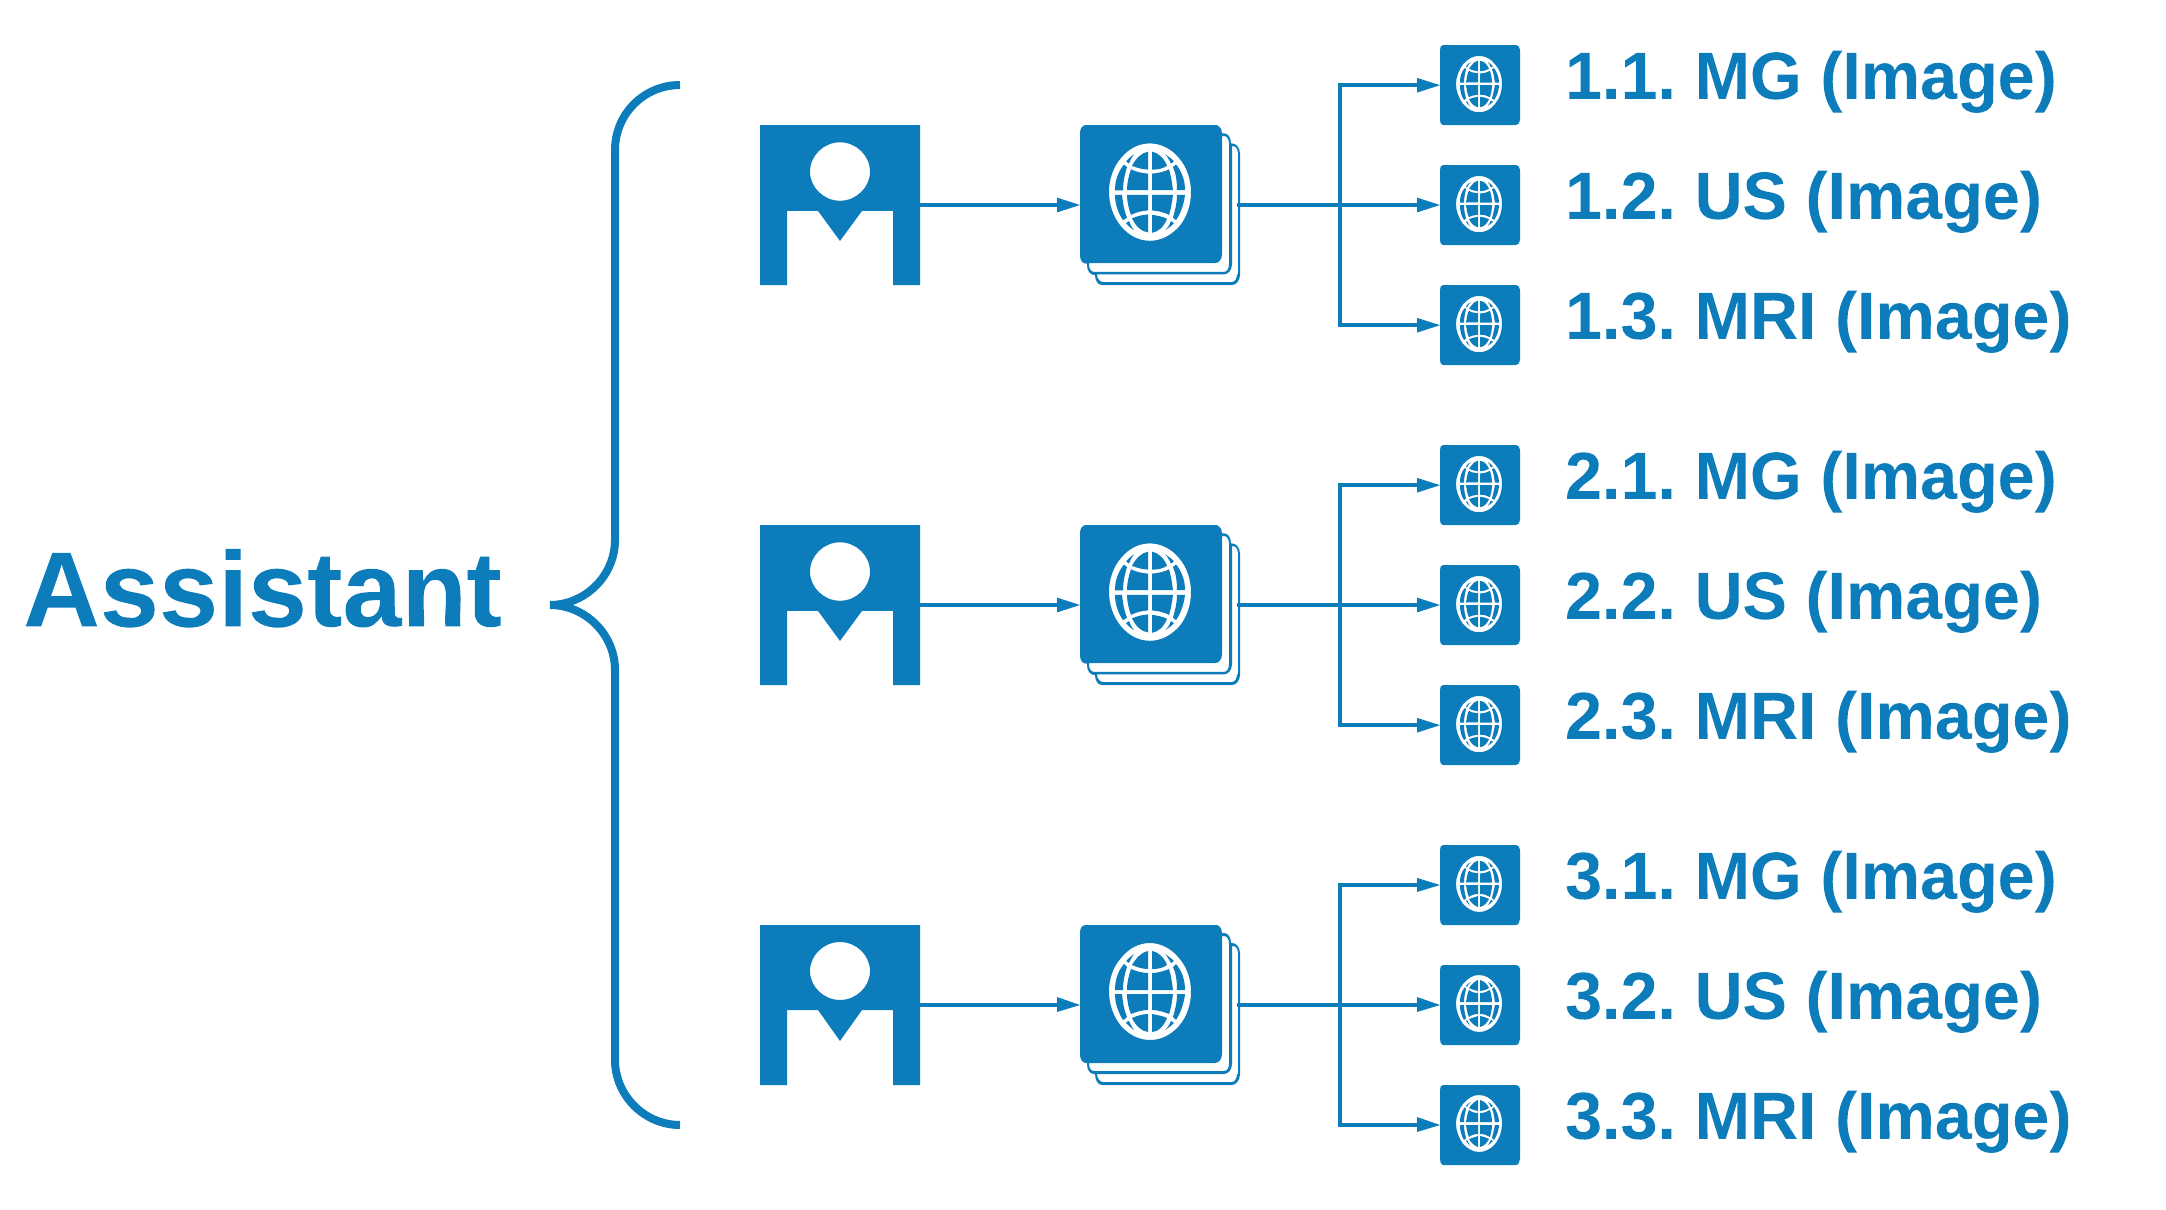
\includegraphics[width=0.50\textwidth]{img001}
\caption{Diagram representing the use of the \textit{Assistant} by clinicians.}
\label{fig:svmm}
\end{wrapfigure}

\hfill

%%%%%%%%%%%%%%%%%%%%%%%%%%%%%%%%%%%%%%%%%%%%%%%%%%%

We will try to understand if, with the \textit{AI-Assisted} techniques, the clinicians will encounters the most accurate severity (\hyperlink{https://en.wikipedia.org/wiki/BI-RADS}{BIRADS}) of the breast lesions~\cite{american1998breast} and patient's prognostic. For this purpose, we have three patients (Figure \ref{fig:svmm}); each patient has three images in the respective modalities: (i) MG; (ii) US; and (iii) MRI. The clinicians will proceed to the activity of diagnosing the three patients within the support of our \textit{Assistant} by the observation of all images.

\hfill

In our \textit{User Testing Guide} a set of tasks is necessary and carefully crafted. Our test studies involve asking participants to perform a set of tasks. By looking at what our user need to do with our system, our tasks are realistic as possible. We are not describing the exact steps participants need to take. We achieve that by avoiding the precise language used as labels in our system. The tasks are emotionally neutrals. And we did several \hyperlink{https://www.nngroup.com/articles/pilot-testing/}{pilot tests} to prevent misleading situations saving us from wasting resources by accidentally use a lousy task or from getting bad data. The tasks are as follows.

The task descriptions below are required to be reviewed by all researchers and facilitators (Section \ref{sec:sec004}) to ensure that the content, format, and presentation are representative of real use and substantially evaluate the total system. Their acceptance is to be documented prior to the user test. Each task, is related to the set of {\it Phases}, {\it Scenarios} and {\it Activities} (Section \ref{sec:sec001}) on the next section (Section \ref{sec:sec008}) further explained.

\clearpage

%%%%%%%%%%%%%%%%%%%%%%%%%%%%%%%%%%%%%%%%%%%%%%%%%%%

List of stand alone tasks for both {\bf Pha1.}, {\bf Pha2.} and {\bf Pha3.} phases:

%%%%%%%%%%%%%%%%%%%%%%%%%%%%%%%%%%%%%%%%%%%%%%%%%%%

\hfill

\begin{itemize}
\item[] \textbf{Task 1.1.1:} Fill the Consent Form (Section \ref{sec:sec001}) and accept the user test;
\item[] \textbf{Task 1.1.2:} Fill the User Characterization Form (Section \ref{sec:sec001}) and proceed;
\end{itemize}

\hfill

\begin{itemize}
\item[] \textbf{Task 2.1.1:} Classify \textit{Patient 1} ({\bf Pat1.}) on the \textit{MM} condition;
\item[] \textbf{Task 2.1.2:} Classify \textit{Patient 2} ({\bf Pat2.}) on the \textit{MM} condition;
\item[] \textbf{Task 2.1.3:} Classify \textit{Patient 3} ({\bf Pat3.}) on the \textit{MM} condition;
\end{itemize}

\hfill

\begin{itemize}
\item[] \textbf{Task 2.2.1:} Freely explore \textit{Patient 1} ({\bf Pat1.}) on the \textit{MM} condition;
\item[] \textbf{Task 2.2.2:} Freely explore \textit{Patient 2} ({\bf Pat2.}) on the \textit{MM} condition;
\item[] \textbf{Task 2.2.3:} Freely explore \textit{Patient 3} ({\bf Pat3.}) on the \textit{MM} condition;
\end{itemize}

\hfill

\begin{itemize}
\item[] \textbf{Task 2.3.1:} Workload \& Usability questions for the \textit{MM} condition;
\item[] \textbf{Task 2.3.2:} {\it Post-task} questions for the \textit{MM} condition;
\end{itemize}

\hfill

\begin{itemize}
\item[] \textbf{Task 3.1.1:} Classify \textit{Patient 1} ({\bf Pat1.}) on the \textit{Assis.} condition;
\item[] \textbf{Task 3.1.2:} Classify \textit{Patient 2} ({\bf Pat2.}) on the \textit{Assis.} condition;
\item[] \textbf{Task 3.1.3:} Classify \textit{Patient 3} ({\bf Pat3.}) on the \textit{Assis.} condition;
\end{itemize}

\hfill

\begin{itemize}
\item[] \textbf{Task 3.2.1:} Freely explore \textit{Patient 1} ({\bf Pat1.}) on the \textit{Assis.} condition;
\item[] \textbf{Task 3.2.2:} Freely explore \textit{Patient 2} ({\bf Pat2.}) on the \textit{Assis.} condition;
\item[] \textbf{Task 3.2.3:} Freely explore \textit{Patient 3} ({\bf Pat3.}) on the \textit{Assis.} condition;
\end{itemize}

\hfill

\begin{itemize}
\item[] \textbf{Task 3.3.1:} Workload \& Usability questions for the \textit{Assis.} condition;
\item[] \textbf{Task 3.3.2:} {\it Post-task} questions for the \textit{Assis.} condition;
\end{itemize}

\hfill

%%%%%%%%%%%%%%%%%%%%%%%%%%%%%%%%%%%%%%%%%%%%%%%%%%%
%%%%%%%%%%%%%%%%%%%%%%%%%%%%%%%%%%%%%%%%%%%%%%%%%%%
%                                                 %
%                     SECTION                     %
%                                                 %
%%%%%%%%%%%%%%%%%%%%%%%%%%%%%%%%%%%%%%%%%%%%%%%%%%%

\section{Metrics}
\label{sec:sec008}

Our user test metrics refers to user performance measured against specific performance goals necessary to satisfy the test requirements. Scenario completion success rates, adherence to dialog scripts, error rates, and subjective evaluations will be used. Time-to-Completion (TtC)~\cite{ioannidis1998effect} of scenarios will also be collected. From the set of tasks (Section \ref{sec:sec007}), each task corresponds to the set of {\it Phases}, {\it Scenarios} and {\it Activities} (Section \ref{sec:sec001}), meaning that we first need to explain it relations.

The first two tasks, {\it i.e.}, {\bf Task 1.1.1} and {\bf Task 1.1.2}, are related to the {\bf Pha1.} phase, as well as with {\bf Act1.}, {\bf Act2.} and {\bf Act3.} activities. The {\bf Pha2.} phase focus on testing and analyzing the {\it \gls{MM}} condition {\it \gls{MM}}, {\it i.e.}, corresponding to {\bf Sce1.} scenario. The six next tasks, {\it i.e.}, {\bf Task 2.1.1}, {\bf Task 2.1.2}, {\bf Task 2.1.3}, {\bf Task 2.2.1}, {\bf Task 2.2.2} and {\bf Task 2.2.3}, are related to {\bf Pha2.} phase. Also, the {\bf Pha2.} phase is related with {\bf Act4.}, {\bf Act5.} and {\bf Act6.} activities, of the {\bf Sce1.} scenario, for diagnosing {\bf Pat1.}, {\bf Pat2.} and {\bf Pat3.} patients. The second next two tasks, {\it i.e.}, {\bf Task 2.3.1} and {\bf Task 2.3.2}, are related with {\bf Act7.} activity of {\bf Pha2.} phase. Now, on the {\bf Pha3.} phase, we will have a relation between testing and analyzing the {\it Assistant (Assis.)} condition, {\it i.e.}, corresponding to {\bf Sce2.} scenario. The six next tasks, {\it i.e.}, {\bf Task 3.1.1}, {\bf Task 3.1.2}, {\bf Task 3.1.3}, {\bf Task 3.2.1}, {\bf Task 3.2.2} and {\bf Task 3.2.3}, are therefore related to {\bf Pha3.} phase. Also, the {\bf Pha3.} phase is related with {\bf Act4.}, {\bf Act5.}, {\bf Act6.} and {\bf Act8.} activities, but this time of the {\bf Sce2.} scenario, for diagnosing {\bf Pat1.}, {\bf Pat2.} and {\bf Pat3.} patients. At the end, the last two tasks, {\it i.e.}, {\bf Task 3.3.1} and {\bf Task 3.3.2}, are related with {\bf Act7.} activity for {\bf Pha3.} phase.

\subsection{Patient Classification}

For the patient classification, we will use the well known scale for classifying the breast cancer disease called \hyperlink{https://en.wikipedia.org/wiki/BI-RADS}{BIRADS}~\cite{balleyguier2007birads}. The \hyperlink{https://en.wikipedia.org/wiki/BI-RADS}{BIRADS} scale is a scheme for putting the findings from breast into a small number of well-defined categories~\cite{obenauer2005applications}.

\hfil

The BIRADS assessment categories are:

\begin{itemize}
\item 0 - Incomplete;
\item 1 - Negative;
\item 2 - Benign Findings;
\item 3 - Probably Benign;
\item 4 - Suspicious Abnormality;
\item 5 - Highly Suspicious of Malignancy;
\item 6 - Known Biopsy Proven Malignancy;
\end{itemize}

For each participant, we will ask the respective examination and respective BIRADS value. From here, we will register the respective value per each scenario, both {\it i.e.}, {\bf Sce1.} and {\bf Sce2.} scenarios. At the end, we can compare the values provided between {\bf Sce1.} and {\bf Sce2.} scenarios. On {\bf Sce1.} scenario, it is where we just improve the visualization technique. Now, with {\bf Sce2.} scenario, {\it i.e.}, an {\it AI-Assistance} diagnosis, we want to understand if the given severity value changed and improved. Also, on {\bf Sce2.} scenario, we want to understand where, {\it i.e.}, on {\it Assistant} or {\it Heatmap} prototype, did the participant took the final improved answer. Nevertheless, we will also compare several other patients' variables, like pathology, to address several other clinical issues.

\subsection{Workload}

To measure the workload, we used the \hyperlink{https://en.wikipedia.org/wiki/NASA-TLX}{NASA Task Load Index (NASA-TLX)}~\cite{ramkumar2017using} scale. The scale is a subjective workload assessment tool that will allow us to perform subjective workload assessments on our participants. For the purpose, we created a repository~\cite{https://doi.org/10.13140/rg.2.2.25301.06883, francisco_maria_calisto_2018_1435044} to cover this need of content.

\hfill

By incorporating a multi-dimensional rating procedure, NASA-TLX derives an overall workload score based on a weighted average of ratings on six sub-scales:

\begin{itemize}
\item Mental Demand
\item Physical Demand
\item Temporal Demand
\item Performance
\item Effort
\item Frustration 
\end{itemize}

At the end, each participant will provide answers regarding the workload information during {\bf Act5.} activity, of {\bf Sce1.} and {\bf Sce2.} scenarios, on both {\bf Pha1.} and {\bf Pha2.} phases respectively. This will also cover both {\bf Task 2.3.1} and {\bf Task 3.3.1} tasks.


\subsection{Usability}

To measure the usability, we used the \hyperlink{https://en.wikipedia.org/wiki/System_usability_scale}{System Usability Scale (SUS)}~\cite{orfanou2015perceived}. The \hyperlink{https://en.wikipedia.org/wiki/System_usability_scale}{SUS} provides a ``quick and dirty", reliable tool for measuring the usability. It consists of a 10 item questionnaire with ten response options for respondents; from {\it Strongly Agree} to {\it Strongly Disagree}. Originally created by John Brooke in 1986, it allows you to evaluate a wide variety of products and services, including hardware, software, mobile devices, websites and applications. For the purpose, we created a repository~\cite{https://doi.org/10.13140/rg.2.2.26978.79044, francisco_maria_calisto_2018_1435042} to cover this need of content.

\hfill

When using \hyperlink{https://en.wikipedia.org/wiki/System_usability_scale}{SUS}, participants are asked to score the following 10 items with one of ten responses that range from {\bf Strongly Agree} to {\bf Strongly Disagree}:

\begin{enumerate}
\item I think that I would like to use this system frequently.
\item I found the system unnecessarily complex.
\item I thought the system was easy to use.
\item I think that I would need the support of a technical person to be able to use this system.
\item I found the various functions in this system were well integrated.
\item I thought there was too much inconsistency in this system.
\item I would imagine that most people would learn to use this system very quickly.
\item I found the system very cumbersome to use.
\item I felt very confident using the system.
\item I needed to learn a lot of things before I could get going with this system.
\end{enumerate}

Again, each participant will provide answers regarding the system's usability information during {\bf Act5.} activity, of {\bf Sce1.} and {\bf Sce2.} scenarios, from both {\bf Pha1.} and {\bf Pha2.} phases respectively. This will also cover both {\bf Task 2.3.1} and {\bf Task 3.3.1} tasks.

\subsection{Predictions}

To measure system predictions with purpose of comparing participants acceptance, we applied our own computational method. The computational method is as follows, while we defined several variables to it, defined next to this information and further explained. Let the {\it Overall Accuracy}~\cite{ashraf2018comparative, li2018digital} be $\O$, a variable following the discrete uniform distribution as $\O \in \mathbb{R}$. The accuracy is used by us to measure how accurate is the overall performance of our solution, considering both positive and negative classes without worrying about data imbalance. Let {\it Total Number of Correct Predictions}~\cite{ashraf2018comparative, li2018digital} be $\tau$, a variable following the discrete uniform distribution as $\tau \in \mathbb{R}$. Let {\it All Possible Predictions}~\cite{ashraf2018comparative, li2018digital} be $\alpha$, a variable following the discrete uniform distribution as $\alpha \in \mathbb{R}$. As follows, we report our computational method.

\hfill

Computational method to measure the {\it Overall Accuracy} of our solution:

\hfill

\begin{Form}
\Large
\begin{center}
$Overall~Accuracy$ = $\frac{Total~Number~of~Correct~Predictions}{All~Possible~Predictions}$
\end{center}
\end{Form}

\hfill

\subsection{Eye Tracking}

Eye movement data was collected for several groups of subjects recruited from the same Portuguese institutions, both public and private, with breast domain-expertise levels, while participants inspected (Section \ref{sec:sec007}) breast images. Medical images will be presented to participants on a monitor (Section \ref{sec:sec005}) attached to a 90Hz eye tracking device, called \hyperlink{https://gaming.tobii.com/product/tobii-eye-tracker-4c/}{Tobii Eye Tracker 4C} with reported accuracy for the collection of eye movement data.

For the eye tracking measurements, we will use the work done by Vaidyana-than et al.~\cite{vaidyanathan2014recurrence}, titled as "{\it Recurrence Quantification Analysis Reveals Eye-Movement Behavior Differences between Experts and Novices}". The work uses eye movement data from medical experts and novices, while they inspected several medical images. Most importantly, the work describe and demonstrate how Recurrence Quantification Analysis (RQA)~\cite{anderson2013recurrence}, and the associated measures, can be used to differentiate eye movement behavior during different viewing conditions and image type finding significant differences. From this work, we aim to use their RQA method to measure and quantify certain eye movement aspects, defined as: (1) Recurrence (REC); (2) Determinism (DET); (3) Laminarity (LAM); and (4) Center Of Recurrence Mass (CORM). We are not yet sure if will use all the presented information, however, the hereby {\it User Testing Guide} serves the purpose of presenting all options for the tests. At this point, we are concern with addressing and collecting the maximum user data as possible.

\subsection{Qualitative Evaluation}

Qualitative and subjective evaluations regarding ease of use and satisfaction will be collected via {\it \hyperlink{https://www.nngroup.com/articles/open-ended-questions/}{open-ended questions}}~\cite{abelson2016supporting, merchant2018digital}, and during debriefing at the conclusion of the session.  The {\it open-ended questions} will utilize free-form responses and feedback, when possible. Whenever possible, it's best to ask {\it \hyperlink{https://www.nngroup.com/articles/open-ended-questions/}{open-ended questions}} so we can find out more than we can anticipate. We will test our questions by trying to answer them with short answers, and rewrite those to find out more about {\it how} and {\it what}. In some cases, we won't be able to accommodate free-form or write-in answers, though, and then it is necessary to limit the possibilities.

\subsection{Scenario Completion}

Each scenario, {\it i.e.}, {\bf Sce1.} and {\bf Sce2.} scenarios, will require, or request, that the participant obtains, or inputs, specific data. This data would be used in course of a typical task. The scenario is completed when the participant indicates the scenario's goal has been obtained. Whether successfully or unsuccessfully. Or the scenario is completed when the participant requests and receives sufficient guidance as to warrant scoring the scenario as a critical error.

\subsection{Time Completion}

The time to complete (ToT)~\cite{delgado2017time, huang2018impact} each scenario, {\it i.e.}, {\bf Sce1.} and {\bf Sce2.} scenarios, not including qualitative and subjective evaluation durations, will be recorded. From this measure, it will be also possible to collect more specific metrics, such as the percentage of time that participants follow an optimal path or the number of times participants need to backtrack.

\subsection{Critical Errors}

Critical Errors are deviations at completion from the targets of the scenario. Obtaining or otherwise reporting of the wrong data value due to participant workflow is a Critical Error. Participants may or may not be aware that the task goal is incorrect or incomplete.

An example of a Critical Error, could be a situation where the participant is not able to open a patient. From this error, we can not even proceed to the next tasks and complete the user test. Despite of the independent completion of the scenario is the goal, we need to guarantee the execution of the test, however, when this errors occur, the facilitator must act.

Critical Errors can also be assigned when the participant initiates, or attempts to initiate, an action that will result in the goal state becoming unobtainable. In general, Critical Errors are unresolved errors preventing completion of the task or errors that produce an incorrect outcome.

\subsection{Non-Critical Errors}

Non-Critical Errors, are errors that are recovered from and by the participant. Or, if not detected, do not result in processing problems or unexpected results. Although Non-Critical Errors can be undetected by the participant, when they are detected they are generally frustrating to the participant.

These errors may be procedural, in which the participant does not complete a scenario in the most optimal means ({\it e.g.}, excessive steps and keystrokes). These errors may also be errors of confusion ({\it e.g.}, initially selecting the wrong function, using a UI control incorrectly such as attempting to edit an un-editable field).

Non-Critical Errors can always be recovered from during the process of completing the scenario. Exploratory behavior, such as opening the wrong menu while searching for a function, will be coded as a non-critical error.
%%%%%%%%%%%%%%%%%%%%%%%%%%%%%%%%%%%%%%%%%%%%%%%%%%%
%                                                 %
%                     SECTION                     %
%                                                 %
%%%%%%%%%%%%%%%%%%%%%%%%%%%%%%%%%%%%%%%%%%%%%%%%%%%

\section{Goals}
\label{sec:sec009}

The next sections will describe the goals for {\it \hyperlink{}{Prototype A Link}}, {\it \hyperlink{}{Prototype B Link}} and {\it \hyperlink{}{Prototype C Link}} prototype expectations. We will try to assess performance-related metrics such as time and correctness of participants completing \textit{tasks} for our expectations. Our expectations are based of the \hyperlink{}{Results Link} obtained at the lab as \hyperlink{https://www.nngroup.com/articles/pilot-testing/}{pilot tests}.

%%%%%%%%%%%%%%%%%%%%%%%%%%%%%%%%%%%%%%%%%%%%%%%%%%%
%                                                 %
%                     SECTION                     %
%                                                 %
%%%%%%%%%%%%%%%%%%%%%%%%%%%%%%%%%%%%%%%%%%%%%%%%%%%

\subsection{Completion Rate}

\textbf{Completion Rate} is the percentage of test participants who successfully complete the task without critical errors. A critical error is defined as an error that results in an incorrect or incomplete outcome. In other words, the completion rate represents the percentage of participants who, when they are finished with the specified task, have an "output" that is correct.

%%%%%%%%%%%%%%%%%%%%%%%%%%%%%%%%%%%%%%%%%%%%%%%%%%%

\hfill

\textit{A \textbf{Completion Rate} of \textbf{90\%} is the goal for each task in this usability test.}

\hfill

%%%%%%%%%%%%%%%%%%%%%%%%%%%%%%%%%%%%%%%%%%%%%%%%%%%

%%%%%%%%%%%%%%%%%%%%%%%%%%%%%%%%%%%%%%%%%%%%%%%%%%%

\hfill

\textbf{Note:} If a participant requires assistance in order to achieve a correct output then the task will be scored as a critical error and the overall completion rate for the task will be affected.

\hfill

%%%%%%%%%%%%%%%%%%%%%%%%%%%%%%%%%%%%%%%%%%%%%%%%%%%

\clearpage

%%%%%%%%%%%%%%%%%%%%%%%%%%%%%%%%%%%%%%%%%%%%%%%%%%%
%                                                 %
%                     SECTION                     %
%                                                 %
%%%%%%%%%%%%%%%%%%%%%%%%%%%%%%%%%%%%%%%%%%%%%%%%%%%

\subsection{Error-Free Rate}

\textbf{Error-Free Rate} is the percentage of test participants who complete the task without any errors (critical or non-critical errors). A non-critical error is an error that would not have an impact on the final output of the task but would result in the task being completed less efficiently.

%%%%%%%%%%%%%%%%%%%%%%%%%%%%%%%%%%%%%%%%%%%%%%%%%%%

\hfill

\textit{An \textbf{Error-Free Rate} of \textbf{80\%} is the goal for each task in this tests.}

\hfill

%%%%%%%%%%%%%%%%%%%%%%%%%%%%%%%%%%%%%%%%%%%%%%%%%%%

%%%%%%%%%%%%%%%%%%%%%%%%%%%%%%%%%%%%%%%%%%%%%%%%%%%
%                                                 %
%                     SECTION                     %
%                                                 %
%%%%%%%%%%%%%%%%%%%%%%%%%%%%%%%%%%%%%%%%%%%%%%%%%%%

\subsection{Time on Task (ToT)}

The time to complete a scenario is referred to as "Time on Task" (ToT). It is measured from the time the participant begins the scenario to the time which the participant signals completion.

%%%%%%%%%%%%%%%%%%%%%%%%%%%%%%%%%%%%%%%%%%%%%%%%%%%
%                                                 %
%                     SECTION                     %
%                                                 %
%%%%%%%%%%%%%%%%%%%%%%%%%%%%%%%%%%%%%%%%%%%%%%%%%%%

\subsection{Subjective Measures}

Subjective opinions about specific tasks, time to perform each task, features, and functionality will be surveyed. At the end of the test, participants will rate their satisfaction with the overall system. Combined with the interview/debriefing session, these data are used to assess attitudes of the participants.

Measuring subjective outcomes based on participants' experiential goals can pose challenges (Section \ref{sec:sec010}) from which an {\it open-ended} flexible approach is catered to personally meaningful goals. On the other hand advocates of formalized User-Centred Design (UCD) goal exploration condemn such informal interviewing as ineffective and we should take it into consideration.

%%%%%%%%%%%%%%%%%%%%%%%%%%%%%%%%%%%%%%%%%%%%%%%%%%%

%%%%%%%%%%%%%%%%%%%%%%%%%%%%%%%%%%%%%%%%%%%%%%%%%%%
%                                                 %
%                     SECTION                     %
%                                                 %
%%%%%%%%%%%%%%%%%%%%%%%%%%%%%%%%%%%%%%%%%%%%%%%%%%%

\subsection{Case Studies}

The functionality of the prototype will be best demonstrated by a series of case studies. By describing the expected workflow and capabilities of the research study at the \textbf{Environment} specific environment and changes of the workflow by using our system prototype. The study implies the evaluation of domain \textit{Scope} features on several domain aspects. The primary goal of this case studies analysis is to generate a receiver operating characteristic to evaluate the performance and validation of our \textit{Scope}. Let us consider a list of hypothetical use cases for the research investigation that evaluates the interaction and usability performance of the \textit{Scope}. Therefore, the following list will show the preliminary case studies.

\clearpage

List of case studies to analyse our solution prototype:

\hfill

\begin{itemize}
\item Case 1;
\item Case 2;
\item Case 3;
\item Case 4;
\end{itemize}

\hfill
%%%%%%%%%%%%%%%%%%%%%%%%%%%%%%%%%%%%%%%%%%%%%%%%%%%
%                                                 %
%                     SECTION                     %
%                                                 %
%%%%%%%%%%%%%%%%%%%%%%%%%%%%%%%%%%%%%%%%%%%%%%%%%%%

\section{Challenges}
\label{sec:sec010}
%%%%%%%%%%%%%%%%%%%%%%%%%%%%%%%%%%%%%%%%%%%%%%%%%%%
%                                                 %
%                     SECTION                     %
%                                                 %
%%%%%%%%%%%%%%%%%%%%%%%%%%%%%%%%%%%%%%%%%%%%%%%%%%%

\section{Results}
\label{sec:sec011}

A \hyperlink{}{Test Report Link} will be provided at the end of this tests. It will consist of a report and/or a presentation of the results; evaluation of the metrics against the pre-approved goals, subjective evaluations, and specific issues of the system, as well as, recommendations for resolution. The recommendations will be categorically sized by development to aid in implementation strategy. The results will be translated to a \hyperlink{}{spreadsheet link} (view only). Also, more related information can be found at \hyperlink{}{Test Link: Test Title}.
%%%%%%%%%%%%%%%%%%%%%%%%%%%%%%%%%%%%%%%%%%%%%%%%%%%
%                                                 %
%                     SECTION                     %
%                                                 %
%%%%%%%%%%%%%%%%%%%%%%%%%%%%%%%%%%%%%%%%%%%%%%%%%%%

\section{Acknowledgements}
\label{sec:sec012}

A special thanks for the support provided by Hugo Lencastre. We would like to thank Doctor Clara Aleluia, Doctor Gisela Andrade, Doctor William Schuitt, Doctor Ana Sofia Germano and Doctor Pedro Marques from the HFF for the generous support and medical expertise. Also, an immense thank for Doctor Cristina Ribeiro da Fonseca. My appreciation goes also to Bruno Cardoso and Bruno Dias for help and above all for the good companionship. Thanks to Professor Daniel Gon\c{c}alves, Professor Daniel Sim\~{o}es Lopes and Daniel Mendes for the technical inputs and network. Last but not least, thank to my advisors Professor Jacinto C. Nascimento and Professor Nuno Jardim Nunes. This work was partially supported by national funds through Funda\c{c}\~{a}o para a Ci\^{e}ncia e a Tecnologia (FCT) with reference UID/CEC/50021/2013 and Instituto Superior T\'{e}cnico (IST-ID) through the FCT/UID/EEA/50009/2013 project, BL89/2017-IST-ID grant. We would like to convey Hospital Fernando Fonseca (HFF) for the collaboration.

\clearpage

\bibliographystyle{plain}
\bibliography{bibliography/references.bib}

\end{document}